\documentclass[]{elsarticle} %review=doublespace preprint=single 5p=2 column
%%% Begin My package additions %%%%%%%%%%%%%%%%%%%
\usepackage[hyphens]{url}

  \journal{Methods in Ecology and Evolution} % Sets Journal name


\usepackage{lineno} % add
  \linenumbers % turns line numbering on
\providecommand{\tightlist}{%
  \setlength{\itemsep}{0pt}\setlength{\parskip}{0pt}}

\usepackage{graphicx}
%%%%%%%%%%%%%%%% end my additions to header

\usepackage[T1]{fontenc}
\usepackage{lmodern}
\usepackage{amssymb,amsmath}
\usepackage{ifxetex,ifluatex}
\usepackage{fixltx2e} % provides \textsubscript
% use upquote if available, for straight quotes in verbatim environments
\IfFileExists{upquote.sty}{\usepackage{upquote}}{}
\ifnum 0\ifxetex 1\fi\ifluatex 1\fi=0 % if pdftex
  \usepackage[utf8]{inputenc}
\else % if luatex or xelatex
  \usepackage{fontspec}
  \ifxetex
    \usepackage{xltxtra,xunicode}
  \fi
  \defaultfontfeatures{Mapping=tex-text,Scale=MatchLowercase}
  \newcommand{\euro}{€}
\fi
% use microtype if available
\IfFileExists{microtype.sty}{\usepackage{microtype}}{}
\bibliographystyle{elsarticle-harv}
\ifxetex
  \usepackage[setpagesize=false, % page size defined by xetex
              unicode=false, % unicode breaks when used with xetex
              xetex]{hyperref}
\else
  \usepackage[unicode=true]{hyperref}
\fi
\hypersetup{breaklinks=true,
            bookmarks=true,
            pdfauthor={},
            pdftitle={A comparison of design-based and model-based approaches for finite population spatial data.},
            colorlinks=false,
            urlcolor=blue,
            linkcolor=magenta,
            pdfborder={0 0 0}}
\urlstyle{same}  % don't use monospace font for urls

\setcounter{secnumdepth}{5}
% Pandoc toggle for numbering sections (defaults to be off)

% Pandoc citation processing
\newlength{\cslhangindent}
\setlength{\cslhangindent}{1.5em}
\newlength{\csllabelwidth}
\setlength{\csllabelwidth}{3em}
% for Pandoc 2.8 to 2.10.1
\newenvironment{cslreferences}%
  {}%
  {\par}
% For Pandoc 2.11+
\newenvironment{CSLReferences}[2] % #1 hanging-ident, #2 entry spacing
 {% don't indent paragraphs
  \setlength{\parindent}{0pt}
  % turn on hanging indent if param 1 is 1
  \ifodd #1 \everypar{\setlength{\hangindent}{\cslhangindent}}\ignorespaces\fi
  % set entry spacing
  \ifnum #2 > 0
  \setlength{\parskip}{#2\baselineskip}
  \fi
 }%
 {}
\usepackage{calc}
\newcommand{\CSLBlock}[1]{#1\hfill\break}
\newcommand{\CSLLeftMargin}[1]{\parbox[t]{\csllabelwidth}{#1}}
\newcommand{\CSLRightInline}[1]{\parbox[t]{\linewidth - \csllabelwidth}{#1}\break}
\newcommand{\CSLIndent}[1]{\hspace{\cslhangindent}#1}

% Pandoc header

\usepackage{bm} \usepackage{bbm} \usepackage{color} \DeclareMathOperator{\var}{{var}} \DeclareMathOperator{\cov}{{cov}} \usepackage{caption} \usepackage{subcaption} \usepackage{setspace} \usepackage{fancyhdr}

\pagestyle{fancy} \fancyhf{} \chead{Spatial design-based vs model-based}
\doublespacing

\begin{document}
\begin{frontmatter}

  \title{A comparison of design-based and model-based approaches for
finite population spatial data.}
    \author[USEPA]{Michael Dumelle\corref{1}}
  
    \author[STLAW]{Matt Higham}
  
    \author[NOAA]{Jay M. Ver Hoef}
  
    \author[USEPA]{Anthony R. Olsen}
  
    \author[OSU]{Lisa Madsen}
  
      \address[USEPA]{United States Environmental Protection Agency, 200
SW 35th St, Corvallis, Oregon, 97333}
    \address[STLAW]{Saint Lawrence University Department of Mathematics,
Computer Science, and Statistics, 23 Romoda Drive, Canton, New York,
13617}
    \address[NOAA]{Marine Mammal Laboratory, Alaska Fisheries Science
Center, National Oceanic and Atmospheric Administration, Seattle,
Washington, 98115}
    \address[OSU]{Oregon State University Department of Statistics, 239
Weniger Hall, Corvallis, Oregon, 97331}
      \cortext[1]{Corresponding Author: Michael Dumelle
(Dumelle.Michael@epa.gov)}
  
  \begin{abstract}
  \begin{enumerate}
  \def\labelenumi{\arabic{enumi}.}
  \tightlist
  \item
    The design-based and model-based approaches to frequentist
    statistical inference rest on fundamentally different foundations.
    In the design-based approach, inference relies on random sampling.
    In the model-based approach, inference relies on distributional
    assumptions. We compare the approaches for finite population spatial
    data.
  \item
    We provide relevant background for the design-based and model-based
    approaches and then study their performance using simulations and an
    analysis of real mercury concentration data. In the simulations, a
    variety of sample sizes, location layouts, dependence structures,
    and response types are considered. In the simualations and real data
    analysis, the population mean is the parameter of interest and
    performance is measured using statistics like bias, squared error,
    and interval coverage.
  \item
    When studying the simulations and mercury concentration data, we
    found that regardless of the strength of spatial dependence in the
    data, sampling plans that incorporate spatial locations (spatially
    balanced samples) generally outperform sampling plans that ignore
    spatial locations (non-spatially balanced samples). We also found
    that model-based approaches tend to outperform design-based
    approaches, even when the data are skewed (and by consequence, the
    model-based distributional assumptions violated). The performance
    gap between these approaches is small when spatially balanced
    samples are used but large when non-spatially balanced samples are
    used. This suggests that the sampling choice (whether to select a
    sample that is spatially balanced) is most important when performing
    design-based inference.
  \item
    There are many benefits and drawbacks to the design-based and
    model-based approaches for finite population spatial data that
    practitioners must consider when choosing between them. We provide
    relevant background contextualizing each approach and study their
    properties in a variety of scenarios, making recommendations for use
    based on the practitioner's goals.
  \end{enumerate}
  \end{abstract}
  
 \end{frontmatter}

\hypertarget{keywords}{%
\section*{Keywords}\label{keywords}}
\addcontentsline{toc}{section}{Keywords}

Design-based inference; Finite Population Block Kriging (FPBK);
Generalized Random Tessellation Stratified (GRTS) algorithm; Local
neighborhood variance estimator; Model-based inference; Restricted
Maximum Likelihood (REML) estimation; Spatially balanced sampling;
Spatial covariance

\hypertarget{sec:introduction}{%
\section{Introduction}\label{sec:introduction}}

When data cannot be collected for all units in a population (i.e.,
population units), data are collected on a subset of the population
units -- this subset is called a sample. There are two general
approaches for using samples to make frequentist statistical inferences
about a population: design-based and model-based. In the design-based
approach, inference relies on randomly assigning some population units
to be in the sample (e.g., random sampling). Alternatively, in the
model-based approach, inference relies on distributional assumptions
about the underlying stochastic process that generated the sample. Each
paradigm has a deep historical context (Sterba, 2009) and its own set of
benefits and drawbacks (Hansen et al., 1983).

Though the design-based and model-based approaches apply to statistical
inference in a broad sense, we focus on comparing these approaches for
spatial data. We define spatial data as data that incorporates the
specific locations of the population units into either the sampling or
estimation process. De Gruijter and Ter Braak (1990) give an early
comparison of design-based and model-based approaches for spatial data,
quashing the belief that design-based approaches could not be used for
spatially correlated data. Since then, there have been several general
comparisons between design-based and model-based approaches for spatial
data (Brus and De Gruijter, 1997; Brus, 2021; Ver Hoef, 2002; Ver Hoef,
2008; Wang et al., 2012). Cooper (2006) reviews the two approaches in an
ecological context before introducing a ``model-assisted'' variance
estimator that combines aspects from each approach. In addition to
Cooper (2006), there has been substantial research and development into
estimators that use both design-based and model-based principles (see
e.g., Sterba (2009) and Cicchitelli and Montanari (2012), and see
Chan-Golston et al. (2020) for a Bayesian approach).

Certainly comparisons between design-based and model-based approaches
have been studied in spatial contexts. But no numerical comparison has
been made between design-based approaches that incorporate spatial
locations into sampling and analysis and model-based approaches. In this
manuscript, we compare design-based approaches that incorporate spatial
locations into sampling and analysis to model-based approaches for
finite population spatial data. A finite population contains a finite
number of population units (we assume the finite number is known); an
example is lakes (treated as a whole with the lake centroid representing
location) in the contiguous United States. Though here we focus on
finite populations, the comparisons we discuss generalize to infinite
populations as well. An infinite population contains an infinite number
of population units; an example is locations within a single lake.

The rest of the manuscript is organized as follows. In Section
\ref{sec:background}, we introduce and provide relevant background for
the design-based and model-based approaches to finite population spatial
data. In Section \ref{sec:mm}, we describe how we compare performance of
the approaches with a simulation study and an analysis of real data that
contains mercury concentration in lakes located in the contiguous United
States. In Section \ref{sec:results}, we present results from the
simulation study and the mercury concentration analysis. And in Section
\ref{sec:discussion}, we end with a discussion and provide directions
for future research.

\hypertarget{sec:background}{%
\subsection{Background}\label{sec:background}}

The design-based and model-based approaches incorporate randomness in
fundamentally different ways. In this section, we describe the role of
randomness for each approach and the subsequent effects on statistical
inferences for spatial data.

\hypertarget{subsec:dvm_compare}{%
\subsubsection{Comparing Design-Based and Model-Based
Approaches}\label{subsec:dvm_compare}}

The design-based approach assumes the population is fixed. Randomness is
incorporated via the selection of population units according to a
sampling design. A sampling design assigns a positive probability of
inclusion (inclusion probability) in the sample to each population unit.
These inclusion probabilities are later used to estimate population
parameters. Some examples of commonly used sampling designs include
simple random sampling, stratified random sampling, and cluster
sampling.

When sampling designs incorporate spatial locations into sampling, we
call the resulting samples ``spatially balanced.'' One approach to
selecting spatially balanced samples is the Generalized Random
Tessellation Stratified (GRTS) algorithm (Stevens and Olsen, 2004),
which we discuss in more detail in Section \ref{subsec:spb_design}. When
sampling designs do not incorporate spatial locations into sampling, we
call the resulting samples ``non-spatially balanced.''

Fundamentally, the design-based approach combines the randomness of the
sampling design with the data collected via the sample to justify the
estimation and uncertainty quantification of fixed, unknown parameters
of a population (e.g., a population mean). Treating the data as fixed
and incorporating randomness through the sampling design yields
estimators having very few other assumptions. Confidence intervals for
these types of estimators are typically derived using limiting arguments
that incorporate all possible samples. Sample means, for example, are
asymptotically normal (Gaussian) by the Central Limit Theorem (under
some assumptions). If we repeatedly select samples from the population,
then 95\% of all 95\% confidence intervals constructed from a procedure
with appropriate coverage will contain the true fixed population mean.
Särndal et al. (2003) and Lohr (2009) provide thorough reviews of the
design-based approach.

The model-based approach assumes the sample is a random realization of a
data-generating stochastic process. Randomness is formally incorporated
through distributional assumptions on this process. Strictly speaking,
randomness need not be incorporated through random sampling, though
Diggle et al. (2010) warn against preferential sampling. Preferential
sampling occurs when the process generating the data locations and the
process being modeled are not independent of one another. To guard
against preferential sampling, model-based approaches often still
implement some form of random sampling. When model-based approaches
implement random sampling, the inclusion probabilities are ignored when
analyzing the sample (in contrast to the design-based approach, which
relies on these inclusion probabilities to analyze the sample).

Instead of estimating fixed, unknown population parameters, as in the
design-based approach, often the goal of model-based inference is to
predict a realized variable, or value. For example, suppose the realized
mean of all population units is the value of interest. Instead of a
fixed, unknown mean, we are the value of the mean, a random variable.
Prediction intervals are then derived using assumptions of the
data-generating stochastic process. If we repeatedly generate response
values from the same process and select samples, then 95\% of all 95\%
prediction intervals constructed from a procedure with appropriate
coverage will contain their respective realized means. Cressie (1993)
and Schabenberger and Gotway (2017) provide thorough reviews of
model-based approaches for spatial data. In Fig. \ref{fig:fig1}, we
provide a visual comparison of the design-based and model-based
approaches (Ver Hoef (2002) and Brus (2021) provide similar figures).

\begin{figure}
  \centering
  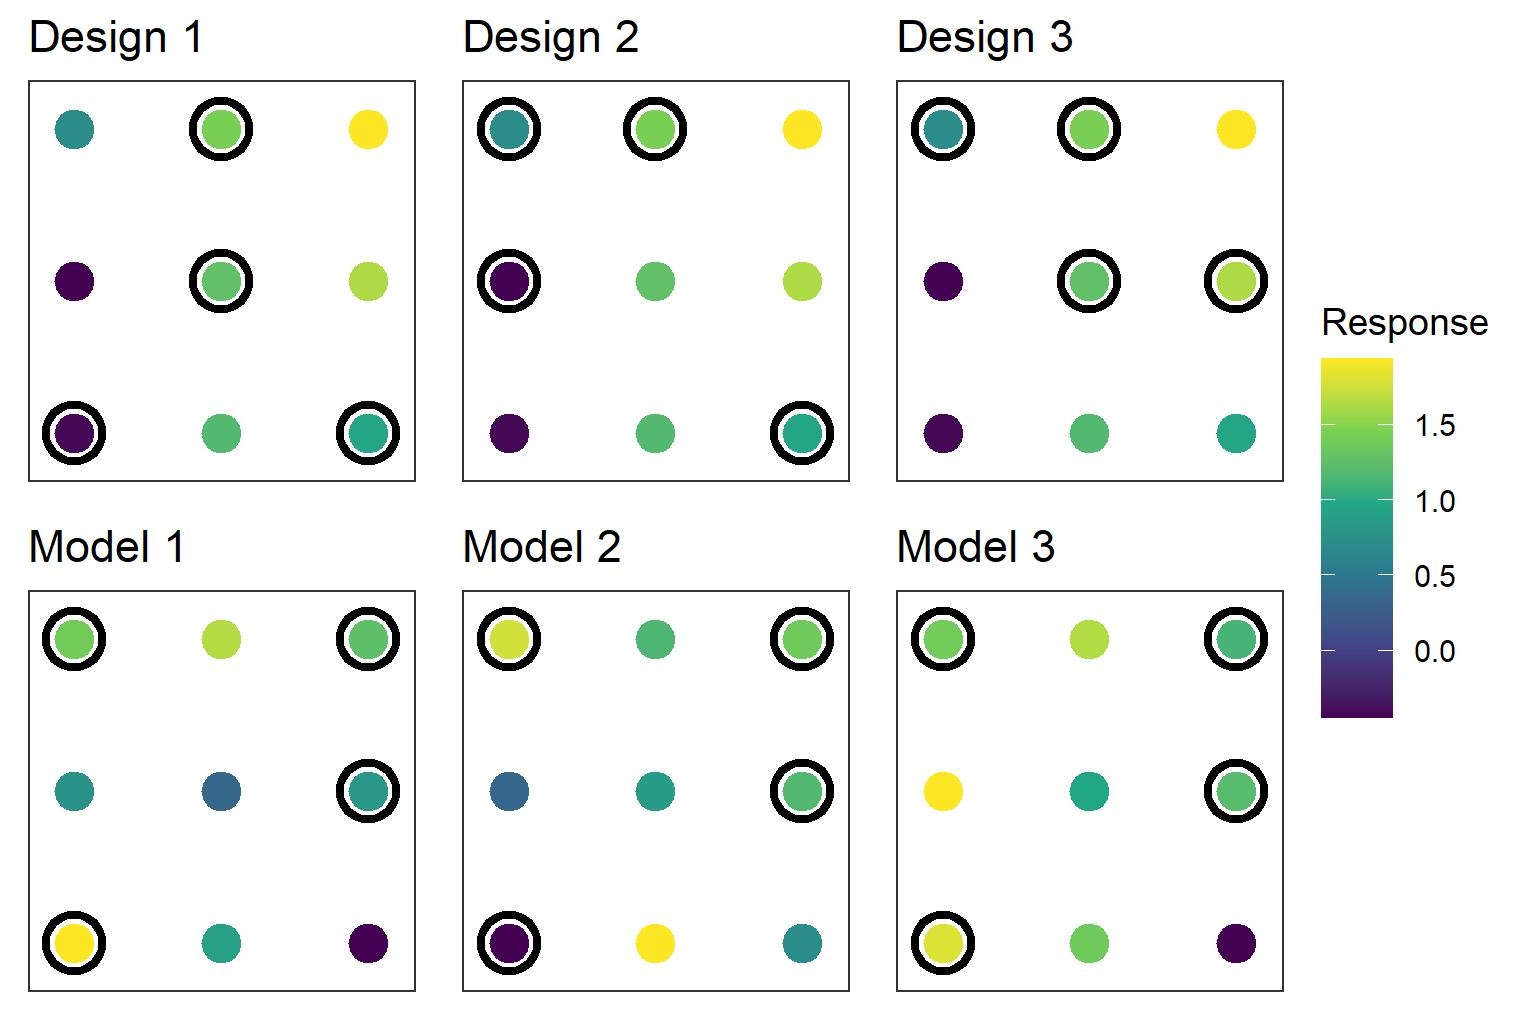
\includegraphics[width = 1\linewidth]{figures/dvm_comp.jpeg}
  \caption{A visual comparison of the design-based and model-based approaches. In the top row, the design-based approach is highlighted. There is one fixed population with nine population units and three random samples of size four (points circled are those sampled). The response values at each site are fixed, but we obtain different estimates for the mean response in each random sample. In the bottom row, the model-based approach is highlighted. There are three realizations of the same data-generating stochastic process that are all sampled at the same four locations. The data-generating stochastic process has a single mean, but the mean of the nine population units is different in each of the three realizations.}
  \label{fig:fig1}
\end{figure}

\hypertarget{subsec:spb_design}{%
\subsubsection{Spatially Balanced Design and
Analysis}\label{subsec:spb_design}}

We previously mentioned that the design-based approach can be used to
select spatially balanced samples (samples that incorporate spatial
locations of the population units). Spatially balanced samples are
useful because parameter estimates from these samples tend to vary less
than parameter estimates from samples that are not spatially balanced
(Barabesi and Franceschi, 2011; Benedetti et al., 2017; Grafström and
Lundström, 2013; Robertson et al., 2013; Stevens and Olsen, 2004; Wang
et al., 2013). The first spatially balanced sampling algorithm to see
widespread use was the Generalized Random Tessellation Stratified (GRTS)
algorithm (Stevens and Olsen, 2004). To quantify the spatial balance of
a sample, Stevens and Olsen (2004) proposed loss metrics based on
Voronoi polygons (Dirichlet Tessellations). After the GRTS algorithm was
developed, several other spatially balanced sampling algorithms emerged,
including the Local Pivotal Method (Grafström et al., 2012; Grafström
and Matei, 2018), Spatially Correlated Poisson Sampling (Grafström,
2012), Balanced Acceptance Sampling (Robertson et al., 2013),
Within-Sample-Distance Sampling (Benedetti and Piersimoni, 2017), and
Halton Iterative Partitioning Sampling (Robertson et al., 2018). In this
manuscript, we select spatially balanced samples using the Generalized
Random Tessellation Stratified (GRTS) algorithm because it has several
attractive properties: the GRTS algorithm accommodates finite and
infinite sampling frames, equal, unequal, and proportional (to size)
inclusion probabilities, legacy (historical) sampling (Foster et al.,
2017), a minimum distance between units in a sample, and replacement
units (replacement units are population units that can be sampled when a
population unit originally selected can no longer be sampled). The GRTS
algorithm selects samples by utilizing a particular mapping between
two-dimensional and one-dimensional space that preserves proximity
relationships. Via this mapping, units in two-dimensional space are
partitioned using a hierarchical address. This hierarchical address is
used to map population units to a one-dimensional line. On the one
dimensional line, each population unit's line length equals its
inclusion probability. Then, a systematic sample of population units is
selected on the line and mapped back to two-dimensional space, yielding
the desired sample. Stevens and Olsen (2004) provide more technical
details.

After selecting a sample and collecting data, unbiased estimates of
population means and totals can be obtained using the Horvitz-Thompson
estimator (Horvitz and Thompson, 1952). If \(\tau\) is a population
total, the Horvitz-Thompson estimator for \(\tau\), denoted by
\(\hat{\tau}_{ht}\), is is given by \begin{align}\label{eq:ht}
  \hat{\tau}_{ht} = \sum_{i = 1}^n Z_i \pi_i^{-1},
\end{align} where \(Z_i\) is the value of the \(i\)th population unit in
the sample, \(\pi_i\) is the inclusion probability of the \(i\)th
population unit in the sample, and \(n\) is the sample size. An estimate
of the population mean is obtained by dividing \(\hat{\tau}_{ht}\) by
\(N\), the number of population units.

It is also important to quantify the uncertainty in \(\hat{\tau}_{ht}\).
Horvitz and Thompson (1952) and Sen (1953) provide variance estimators
for \(\hat{\tau}_{ht}\), but these estimators have two drawbacks. First,
they rely on calculating \(\pi_{ij}\), the probability that population
unit \(i\) and population unit \(j\) are both in the sample -- this
quantity can be challenging if not impossible to calculate analytically.
Second, these estimators ignore the spatial locations of the population
units. To address these two drawbacks simultaneously, Stevens and Olsen
(2003) proposed the local neighborhood variance estimator. The local
neighborhood variance estimator does not rely on \(\pi_{ij}\) and
incorporates spatial locations -- for technical details see Stevens and
Olsen (2003). Stevens and Olsen (2003) show the local neighborhood
variance estimator tends to reduce the estimated variance of
\(\hat{\tau}\) and yield more precise (narrower) confidence intervals
compared to variance estimators that ignore spatial locations.

\hypertarget{finite-population-block-kriging}{%
\subsubsection{Finite Population Block
Kriging}\label{finite-population-block-kriging}}

Finite Population Block Kriging (FPBK) is a model-based approach that
expands the geostatistical Kriging framework to the finite population
setting (Ver Hoef, 2008). Instead of developing inference based on a
specific sampling design, we assume the data are generated by a spatial
stochastic process. We summarize some of the basic principles of FBPK
next -- for technical details, see Ver Hoef (2008). Let
\({\mathbf{z} \equiv \{\text{z}(s_1), \text{z}(s_2), . . . , \text{z}(s_N) \}}\)
be an \(N \times 1\) response vector at locations \(s_1\), \(s_2\), . .
. , \(s_N\) that can be measured at the \(N\) population units. Suppose
we want to use a sample to predict some linear function of the response
variable, \(f(\mathbf{z}) = \mathbf{b}^\prime \mathbf{z}\), where
\(\mathbf{b}^\prime\) is a \(1 \times N\) vector of weights (e.g, the
population mean is represented by a weights vector whose elements all
equal \(1 / N\)). Denoting quantities that are part of the sampled
population units with a subscript \emph{s} and quantities that are part
of the unsampled population units with a subscript \emph{u}, let

\begin{equation}
\begin{pmatrix} \label{equation:Zmarginal}
    \mathbf{z}_s      \\
    \mathbf{z}_u
\end{pmatrix}
=
\begin{pmatrix}
  \mathbf{X}_s    \\
  \mathbf{X}_u
\end{pmatrix}
\bm{\beta} +
\begin{pmatrix}
\bm{\delta}_s    \\
\bm{\delta}_u
\end{pmatrix},
\end{equation} where \(\mathbf{X}_s\) and \(\mathbf{X}_u\) are the
design matrices for the sampled and unsampled population units,
respectively, \(\bm{\beta}\) is the parameter vector of fixed effects,
and \(\bm{\delta} \equiv [\bm{\delta}_s \,\, \bm{\delta}_u]'\), where
\(\bm{\delta}_s\) and \(\bm{\delta}_u\) are random errors for the
sampled and unsampled population units, respectively.

FBPK assumes \(\bm{\delta}\) in Equation\(~\)\ref{equation:Zmarginal}
has mean-zero and a spatial dependence structure that can be modeled
using a covariance function. This covariance function is commonly
assumed to be non-negative, second-order stationary (depending only on
the distance between population units), isotropic (independent of
direction), and decay with distance between population units (Cressie,
1993). Henceforth, it is implied that we have made these same
assumptions regarding \(\bm{\delta}\), though Chiles and Delfiner
(1999), pp.~80-93 discuss covariance functions that are not second-order
stationary, not isotropic, or not either. A variety of flexible
covariance functions can be used to model \(\bm{\delta}\) (Cressie,
1993); one example is the exponential covariance function (Cressie
(1993) provides a thorough list of spatial covariance functions). The
\(i,j\)th element of the exponential covariance matrix,
\(\mathop{\mathrm{{cov}}}(\bm{\delta})\), is \mbox{}
\begin{align}\label{equation:expcov}
\mathop{\mathrm{{cov}}}(\delta_i, \delta_j) = 
\begin{cases} 
\sigma^2_{1}\exp(-h_{i,j}/\phi) & h_{i,j} > 0 \\
\sigma^2_{1} + \sigma^2_2 & h_{i,j} = 0
\end{cases}
,
\end{align} where \(\sigma^2_{1}\) is the variance parameter quantifying
the variability that is dependent (coarse-scale), \(\sigma^2_{2}\) is
the variance parameter quantifying the variability that is independent
(fine-scale), \(\phi\) is the range parameter measuring the
distance-decay rate of the covariance, and \(h_{i,j}\) is the Euclidean
distance between population units \(i\) and \(j\). The proportion of
variability attributable to dependent random error is
\(\sigma^2_{1} / (\sigma^2_{1} + \sigma^2_{2})\). Similarly, the
proportion of variability attributable to independent random error is
\(\sigma^2_{2} / (\sigma^2_{1} + \sigma^2_{2})\). Finally we note that
\(\sigma^2_{1}\) and \(\sigma^2_{2}\) are often called the partial sill
and nugget, respectively.

With the above model formulation, the Best Linear Unbiased Predictor
(BLUP) for \(f(\mathbf{b}'\mathbf{z})\) and its prediction variance can
be computed. While details of the derivation are in Ver Hoef (2008), we
note here that the predictor and its variance are both moment-based,
meaning that they do not rely on any distributional assumptions.
Distributional assumptions are used, however, when constructing
prediction intervals.

Other approaches, such as k-nearest-neighbors (Fix and Hodges, 1989; Ver
Hoef and Temesgen, 2013) and random forest (Breiman, 2001), among
others, could also be used to obtain predictions for a mean or total
from finite population spatial data. Compared to the k-nearest-neighbors
and random forest approach, we prefer FBPK because it is model-based and
relies on theoretically-based variance estimators leveraging the model's
spatial covariance structure, whereas k-nearest-neighbors and random
forests use ad-hoc variance estimators (Ver Hoef and Temesgen, 2013).
Additionally, Ver Hoef and Temesgen (2013) studied compared FBPK,
k-nearest-neighbors, and random forest in a variety of spatial data
contexts, and FBPK tended to perform best.

\hypertarget{sec:mm}{%
\section{Materials and Methods}\label{sec:mm}}

\hypertarget{sec:mm_sim}{%
\subsection{Simulation Study}\label{sec:mm_sim}}

We used a simulation study to investigate performance of four
sampling-analysis combinations. The first sampling-analysis combination
was IRS-Design. In IRS-Design, samples were selected with the
Independent Random Sampling (IRS) algorithm. The IRS algorithm ignores
the spatial locations of the population units, thus the IRS samples were
not spatially balanced. In IRS-Design, samples were analyzed using the
design-based approach via the Horvitz-Thompson mean estimator and an IRS
variance estimator that ignored the spatial locations of the units in
the sample. The second sampling-analysis combination was IRS-Model,
where samples were selected with the IRS algorithm and analyzed using
the model-based approach via Restricted Maximum Likelihood (REML)
estimation (Harville, 1977; Patterson and Thompson, 1971; Wolfinger et
al., 1994). The third sampling-analysis combination was GRTS-Design,
where samples were selected with the GRTS algorithm and analyzed using
the design-based approach via the Horvitz-Thompson mean estimator and
the local neighborhood variance estimator (which does incorporate the
spatial locations of the units in the sample). The fourth and final
sampling-analysis combination was GRTS-Model, where samples were
selected with the GRTS algorithm and analyzed using the model-based
approach via REML estimation. These sampling-analysis combinations are
also provided in Table \ref{tab:designanalysis}. Lastly we note that for
both the IRS and GRTS samples, equal inclusion probabilities were
assumed for all population units. When IRS assumes equal inclusion
probabilities for all population units, the algorithm is equivalent to
simple random sampling (SRS).

\begin{table}[ht]
\centering
\begin{tabular}{r|ll}
  \hline
 & Design & Model \\ 
  \hline
IRS & IRS-Design & IRS-Model \\ 
  GRTS & GRTS-Design & GRTS-Model \\ 
   \hline
\end{tabular}
\caption{\label{tab:designanalysis} Sampling-analysis combinations in the simulation study. The rows give the two types of sampling designs and the columns give the two types of analyses.} 
\end{table}

Performance for the four sampling-analysis combinations was evaluated in
36 different simulation scenarios. The 36 scenarios resulted from the
crossing of three sample sizes, two location layouts (of the population
units), two response types, and three proportions of dependent random
error. The three sample sizes (\(n\)) were \(n = 50, n = 100,\) and
\(n = 200\). Samples were always selected from a population size (\(N\))
of \(N = 900\). The two location layouts were random and gridded.
Locations in the random layout were randomly generated inside the unit
square (\([0, 1] \times [0, 1]\)). Locations in the gridded layout were
placed on a fixed, equally spaced grid inside the unit square. The two
response types were normal and lognormal. For the normal response type,
the response was simulated using mean-zero random errors with the
exponential covariance (Equation\(~\)\ref{equation:expcov}) for varying
proportions of dependent random error. The proportion of dependent
random error is represented by
\(\sigma^2_1 / (\sigma^2_1 + \sigma^2_2)\), where \(\sigma^2_1\) and
\(\sigma^2_2\) are the dependent random error variance (partial sill)
and independent random error variance (nugget) from
Equation\(~\)\ref{equation:expcov}, respectively. The total variance,
\(\sigma^2_1 + \sigma^2_2\), was always 2. The range was always
\(\sqrt{2} / 3\), chosen so that the correlation in the dependent random
error decayed to nearly zero at \(\sqrt{2}\), the largest possible
distance between two population units in the domain. For the lognormal
response type, the response was first simulated using the same approach
as for the normal response type, except that the total variance was
0.6931 instead of 2. The response was then exponentiated, yielding a
lognormal random variable whose total variance was 2. The lognormal
responses were used to evaluate performance of the sampling-analysis
approaches for data that were skewed (i.e., not normal).

\begin{table}[ht]
\centering
\begin{tabular}{r|lll}
   \hline
Sample Size (n) & 50 & 100 & 200 \\ 
  Location Layout & Random & Gridded & - \\ 
  Proportion of Dependent Error & 0 & 0.5 & 0.9 \\ 
  Response Type & Normal & Lognormal & - \\ 
   \hline
\end{tabular}
\caption{\label{tab:parmtab} Simulation scenario options. All combinations of sample size, location layout, response type, and proportion of dependent random error composed the 36 simulation scenarios. In each simualtion scenario, the total variance was 2.} 
\end{table}

In each of the 36 simulation scenarios, there were 2000 independent
simulation trials. In each trial, IRS and GRTS samples were selected and
then design-based and model-based analyses were used to estimate
(design-based) or predict (model-based) the mean and construct 95\%
confidence (design-based) or 95\% prediction (model-based) intervals.
Then we recorded the bias, squared error, standard error, and interval
coverage for all sampling-analysis combinations. After all 2000 trials,
we summarized the long-run performance of the combinations by
calculating mean bias, rMS(P)E (root-mean-squared error for the
design-based approaches and root-mean-squared-prediction error for the
model-based approaches), MStdE (mean standard error), and the proportion
of times the true mean is contained in its 95\% confidence
(design-based) or 95\% prediction (model-based) interval. The 95\%
intervals were constructed using the normal distribution. Justification
for this comes from the asymptotic normality of means via the Central
Limit Theorem (under some assumptions). Quantifying mean bias and
rMS(P)E is important because they help us understand how far (under
different loss metrics) the estimates (design-based) or predictions
(model-based) tend to be from the true mean. Quantifying MStdE is
important because it helps us understand how precise intervals tend to
be. Quantifying interval coverage is important because it helps us
understand how often our 95\% intervals actually contain the true mean.

The IRS algorithm, IRS variance estimator, GRTS algorithm, and local
neighborhood variance estimator are available in the \texttt{spsurvey}
\textbf{\textsf{R}} package (Dumelle et al., 2021). FPBK is available in
the \texttt{sptotal} \textbf{\textsf{R}} package (Higham et al., 2021).

\hypertarget{sec:mm_app}{%
\subsection{Application}\label{sec:mm_app}}

The United States Environmental Protection Agency (USEPA), states, and
tribes periodically conduct National Aquatic Research Surveys (NARS) to
assess the water quality of various bodies of water in the contiguous
United States. One component of NARS is the National Lakes Assessment
(NLA), which measures various aspects of lake health and water quality
(USEPA, 2012). We will analyze mercury concentration data collected at
986 lakes from the 2012 NLA. Although we can calculate the true mean
mercury concentration values for these 986 lakes, here we will explore
whether or not we can obtain an adequately precise estimate
(design-based) or prediction (model-based) for the realized mean mercury
concentration if we sample only 100 of the 986 lakes. For each of the
four familiar sampling-analysis combinations (IRS-Design, IRS-Model,
GRTS-Design, and GRTS-Model), we estimate (design-based) or predict
(model-based) the mean mercury concentration and construct 95\%
intervals from this sample of 100 lakes and compare to the true mean
mercury concentration from all 986 lakes.

\hypertarget{sec:results}{%
\section{Results}\label{sec:results}}

\hypertarget{sec:r_sim}{%
\subsection{Simulation Study}\label{sec:r_sim}}

The mean bias was nearly zero for all four sampling-analysis
combinations in all 36 scenarios, so we omit a more detailed summary of
those results here. Tables for mean bias in all 36 simulation scenarios
are provided in the supporting information.

Fig. \ref{fig:rmspe_eff} shows the relative rMS(P)E of the four sampling
analysis combinations using the random location layout with
``IRS-Design'' as the baseline. The relative rMS(P)E is defined as
\begin{equation*}
\frac{\text{rMS(P)E of sampling-analysis combination}}{\text{rMS(P)E of IRS-Design}},
\end{equation*} When there is no spatial covariance (Fig.
\ref{fig:rmspe_eff}, ``Prop DE: 0'' row), the four sampling-analysis
combinations have approximately equal rMS(P)E and using the GRTS
algorithm or a model-based analysis does not result in much, if any,
loss in efficiency compared to IRS-Design. When there is spatial
covariance (Fig. \ref{fig:rmspe_eff}, ``Prop DE: 0.5'' and ``Prop DE:
0.9'' rows), GRTS-Model tends to have the lowest rMS(P)E, followed by
GRTS-Design, IRS-Model, and finally IRS-Design, though the difference in
relative rMS(P)E among GRTS-Model, GRTS-Design, and IRS-Model is
relatively small. As the strength of spatial covariance increases, the
gap in rMS(P)E between IRS-Design and the other sampling-analysis
combinations widens. Finally we note that when there is spatial
covariance, IRS-Model has a much lower rMS(P)E than IRS-Design,
suggesting that the poor design properties of IRS are largely mitigated
by the model-based analysis. These rMS(P)E conclusions are similar to
those observed in the grid location layout, so we omit a grid location
layout figure here. Tables for rMS(P)E in all 36 simulation scenarios
are provided in the supporting information.

\begin{figure}
  \centering
  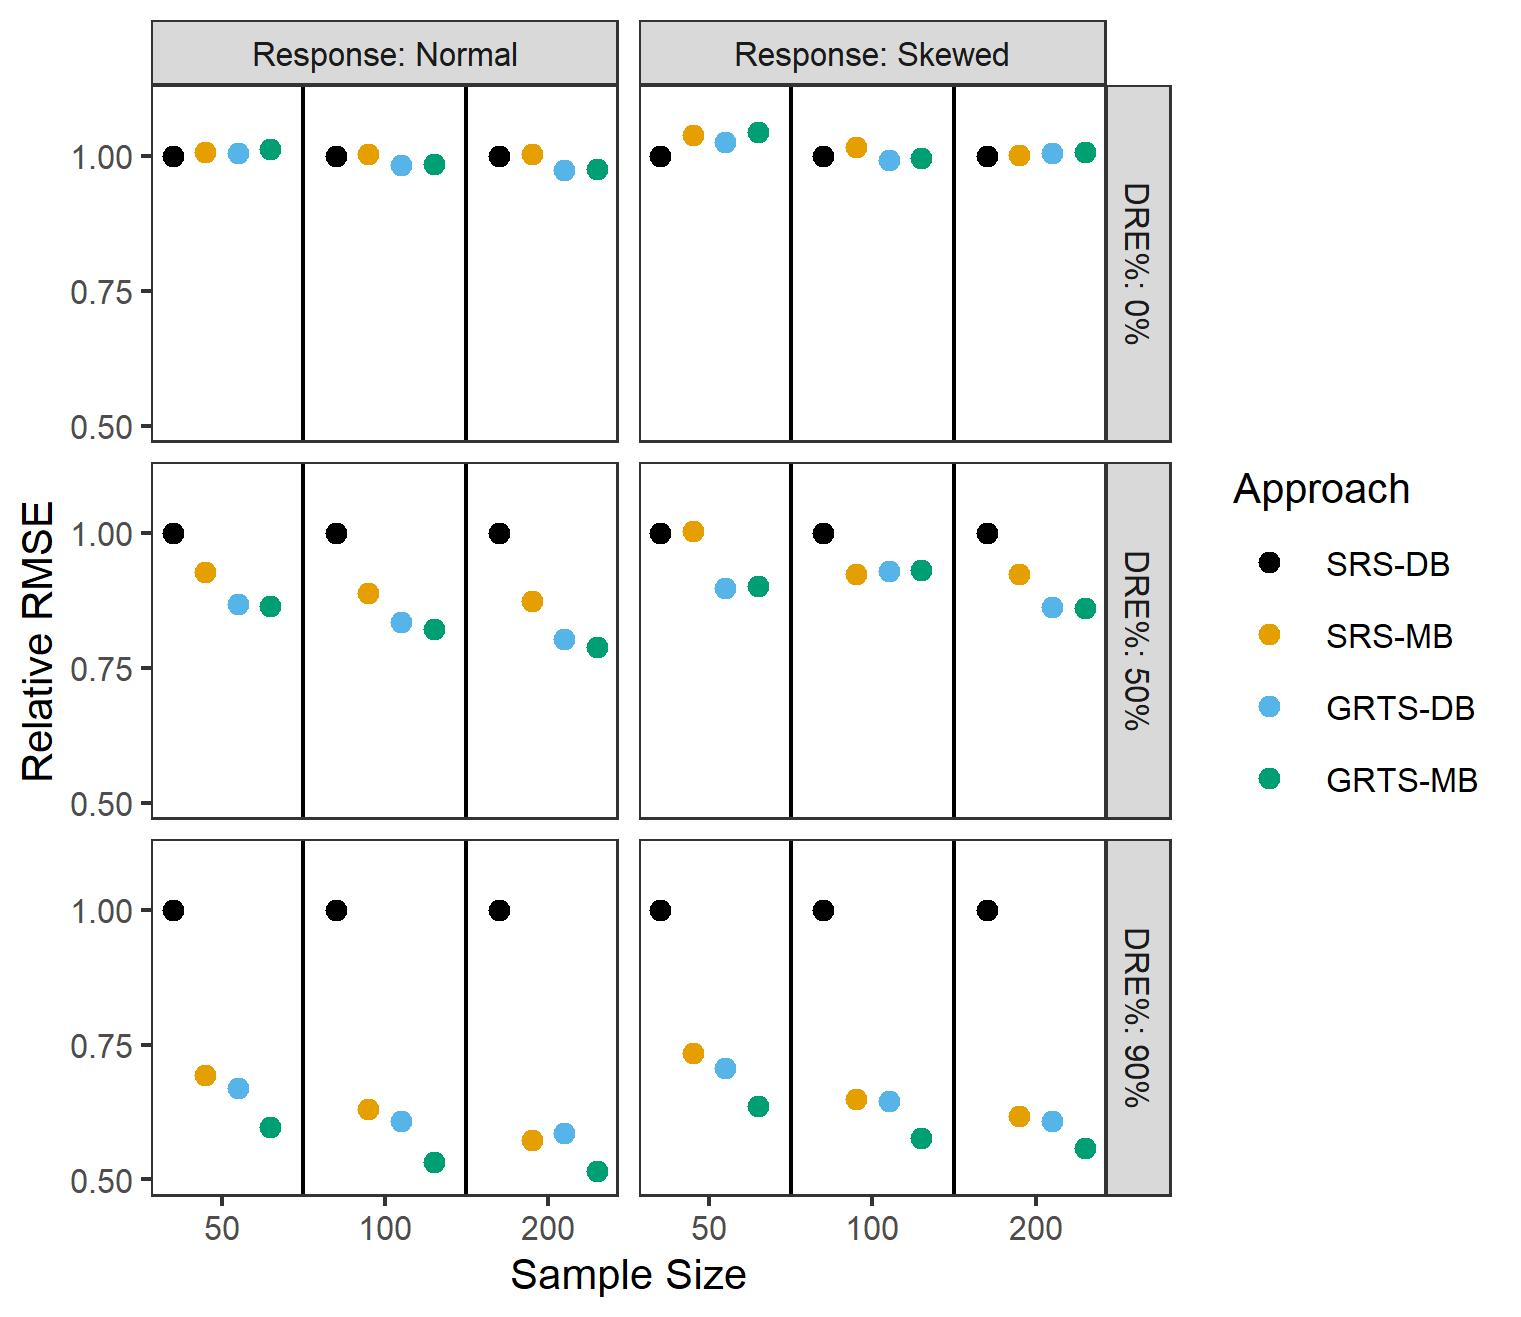
\includegraphics[width = 1\linewidth]{figures/rmspe_eff.jpeg}
  \caption{Relative rMS(P)E in the simulation study for the four sampling-analysis combinations. The rows indicate the proportion of dependent error and the columns indicate the response type.}
  \label{fig:rmspe_eff}
\end{figure}

Fig. \ref{fig:mse_eff} shows the relative MStdE of the four
sampling-analysis combinations using the random location layout with
``IRS-Design'' as the baseline. The relative MStdE is defined as
\begin{equation*}
\frac{\text{MStdE of sampling-analysis combination}}{\text{MStdE of IRS-Design}},
\end{equation*} Many general takeaways regarding MStdE are similar to
general takeaways regarding rMS(P)E: there seems to be no benefit to
using IRS, even when there is no spatial covariance; as the strength of
spatial covariance increases, the gap in MStdE between IRS-Design and
the other sampling-analysis combinations widens; and IRS-Model
outperforms IRS-Design by a noticeable margin. These fact that the
rMS(P)E and MStdE findings are similar is not particularly surprising
because the mean bias for all sampling-analysis combinations was nearly
zero, thus rMS(P)E is driven by the standard error of the estimators
(design-based) or predictors (model-based). We do note that between
GRTS-Design and GRTS-Model, GRTS-Design had lower MStdE when there was
no spatial covariance or a medium amount of spatial covariance (Fig.
\ref{fig:mse_eff}, ``Prop DE: 0'' and ``Prop DE: 0.5'' rows), and
GRTS-Model had lower MStdE when there was a high amount of spatial
covariance (Fig. \ref{fig:mse_eff}, ``Prop DE: 0.9'' row). These MStdE
conclusions are similar to those observed in the grid location layout,
so we omit a grid location layout figure here. Tables for MStdE in all
36 simulation scenarios are provided in the supporting information.

\begin{figure}
  \centering
  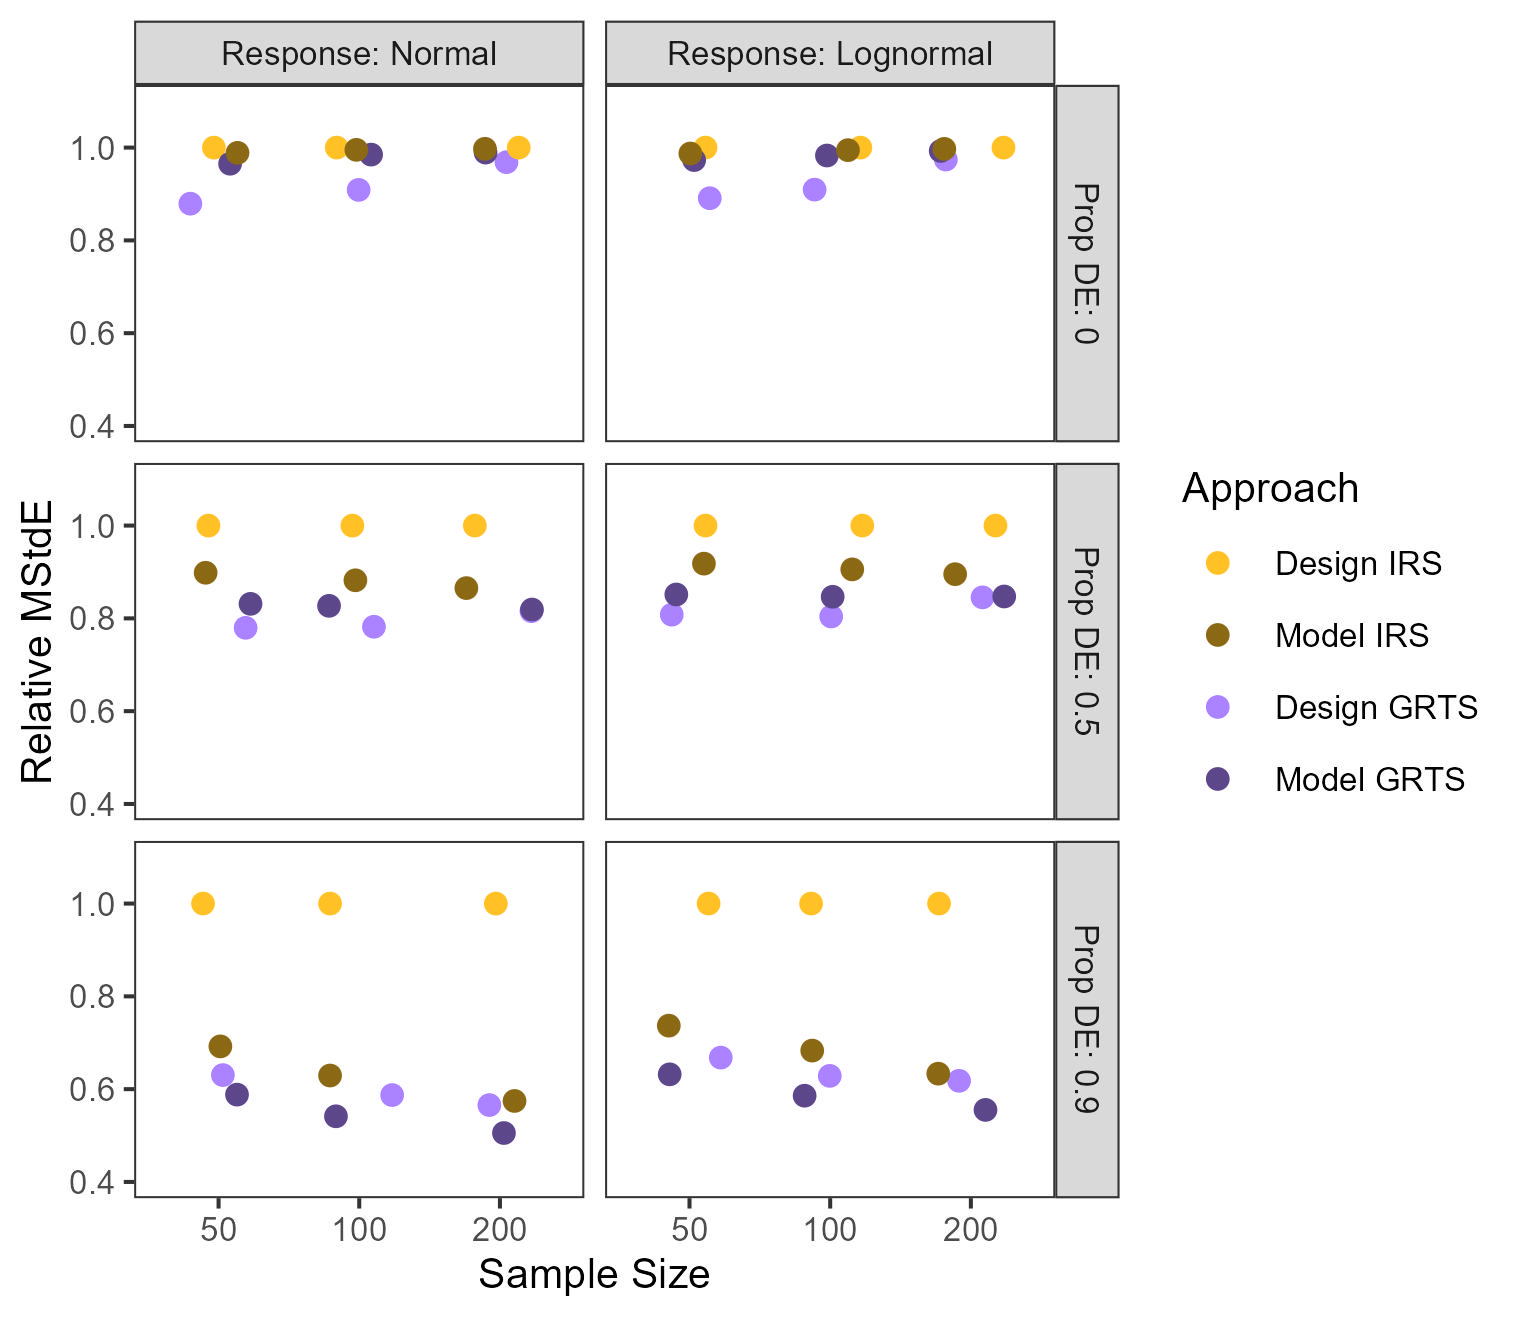
\includegraphics[width = 1\linewidth]{figures/mse_eff.jpeg}
  \caption{Relative MStdE in the simulation study for the four sampling-analysis combinations. The rows indicate the proportion of dependent error and the columns indicate the response type.}
  \label{fig:mse_eff}
\end{figure}

Fig. \ref{fig:figconf} shows the 95\% interval coverage for each of the
four sampling-analysis combinations in the random location layout.
Within each scenario, the sampling-analysis combinations tend to have
fairly similar interval coverage, though when \(n = 50\) or \(n = 100\),
GRTS-Design coverage is usually a few percentage points lower than the
other combinations. Coverage in the normal response scenarios was
usually near 95\%, while coverage in the lognormal response scenarios
usually varied from 90\% to 95\% but increased with the sample size. At
a sample size of 200, all four sampling-analysis combinations had
approximately 95\% interval coverage in both response scenarios for all
dependent error proportions. These interval coverage conclusions are
similar to those observed in the grid location layout, so we omit a grid
location layout figure here. Tables for interval coverage in all 36
simulation scenarios are provided in the supporting information.

\begin{figure}
  \centering
  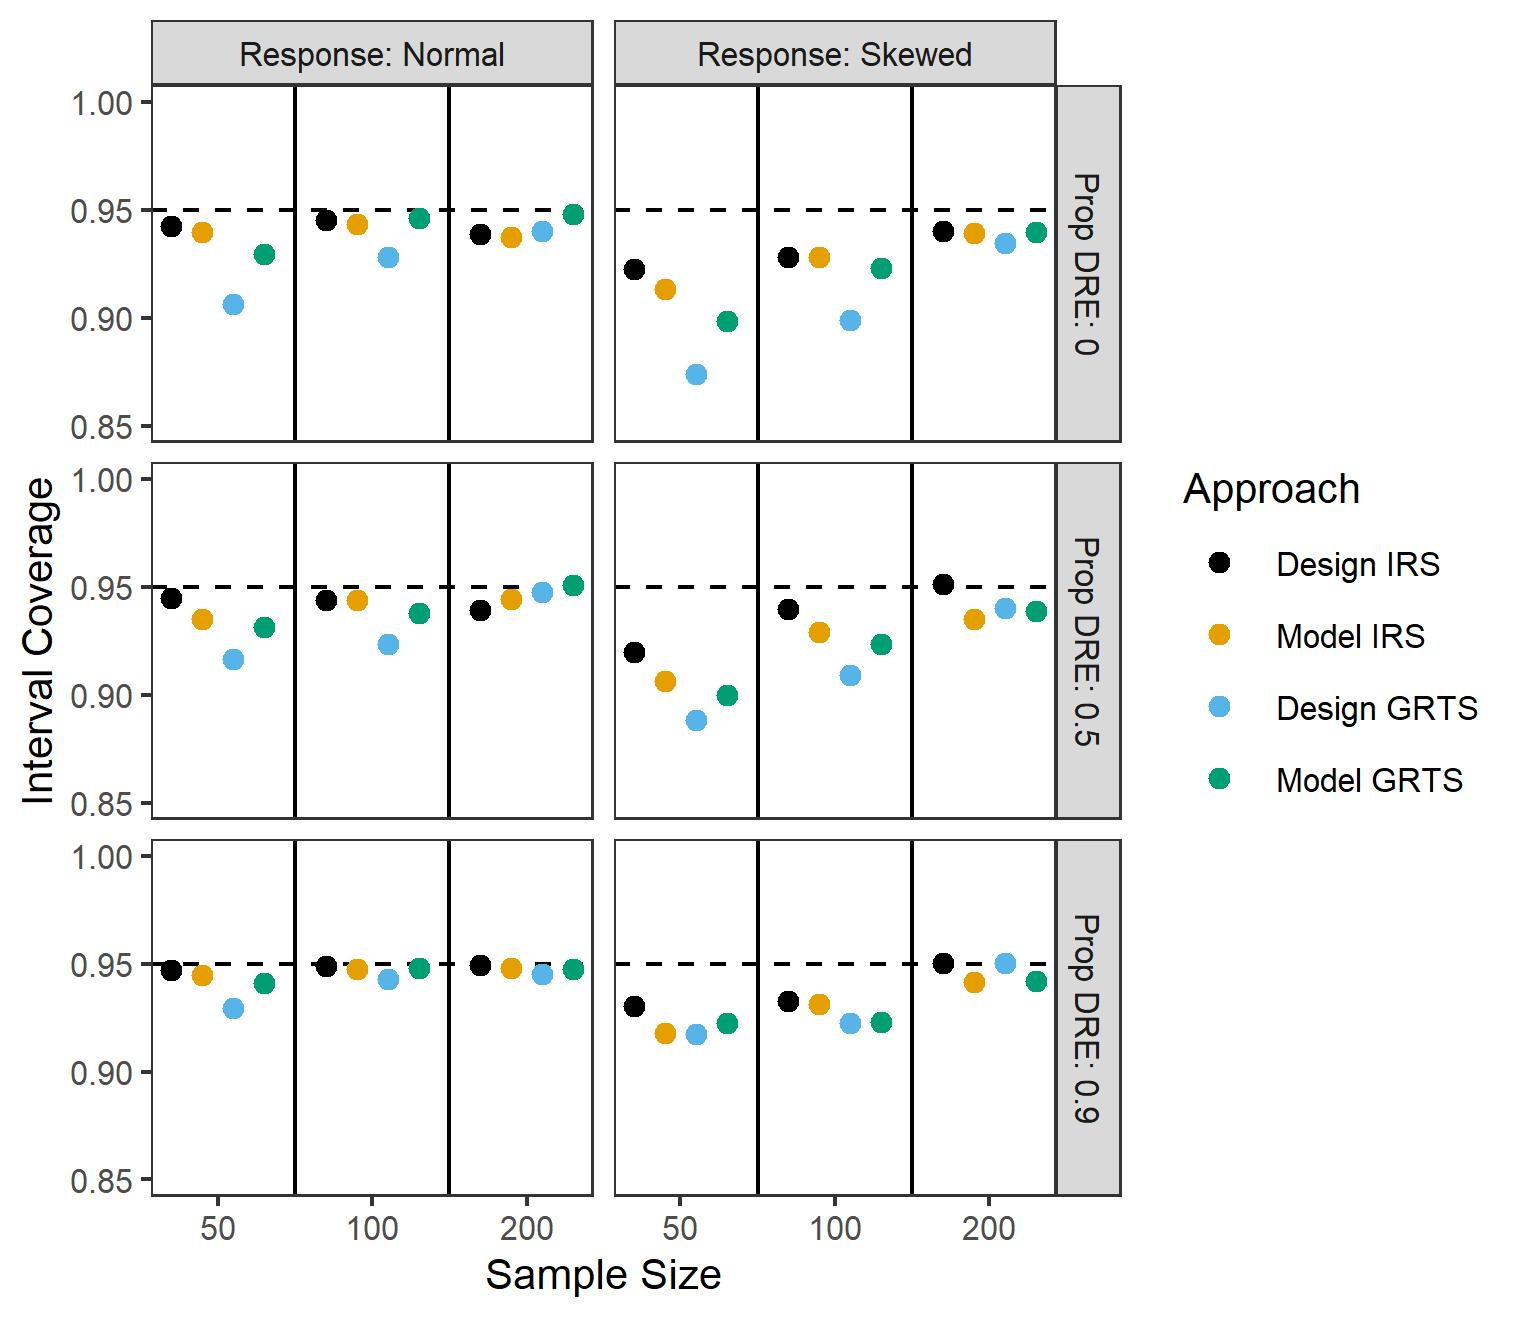
\includegraphics[width = 1\linewidth]{figures/coverage.jpeg}
  \caption{Interval coverage in the simulation study for the four sampling-analysis combinations. The rows indicate the proportion of dependent error and the columns indicate the response type. The solid, black line represents 95\% coverage.}
  \label{fig:figconf}
\end{figure}

\hypertarget{sec:r_app}{%
\subsection{Application}\label{sec:r_app}}

Fig. \ref{fig:merc} shows a map and histogram of mercury concentration
in all 986 NLA lakes. The map shows mercury concentration exhibits some
spatial patterning, with high mercury concentrations in the northeast
and north central United States. The histogram shows that mercury
concentration is right-skewed, with most lakes having a low value of
mercury concentration but a few having a much higher concentration. Fig.
\ref{fig:merc} also shows mercury concentration's empirical
semivariogram. The empirical semivariogram can be used as a tool to
visualize spatial dependence. It quantifies the mean of the halved
squared differences (semivariance) among all pairs of mercury
concentrations at different distances apart. When a process has spatial
covariance (exhibits spatial dependence), the mean semivariance tends to
be smaller at small distances and larger at large distances. The
empirical semivariogram in Fig. \ref{fig:merc} suggests that mercury
concentration exhibits spatial dependence. Lastly we note that the true
mean mercury concentration in the 986 NLA lakes is 103.2 ng / g.

\begin{figure}
\centering
\begin{subfigure}{0.98\textwidth}
  \centering
  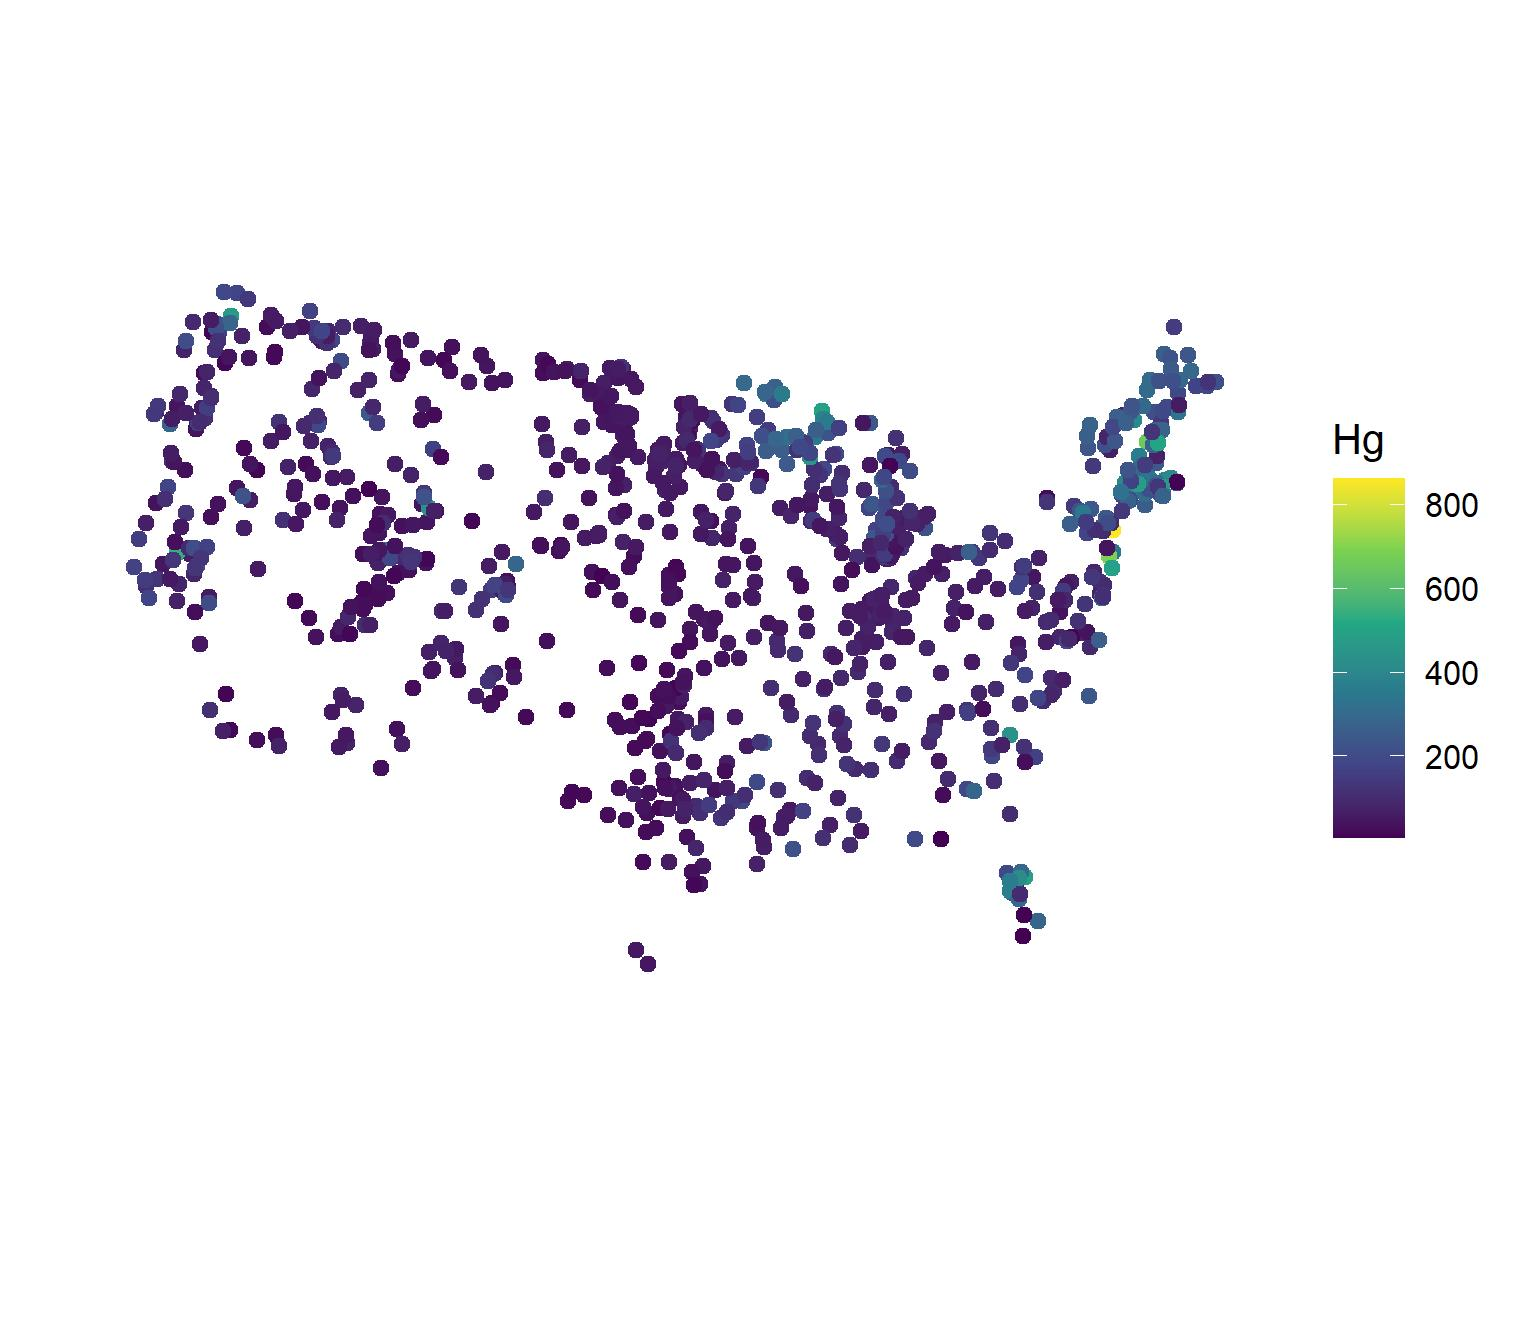
\includegraphics[width = 1\linewidth]{figures/mercury_map.jpeg}
  \caption*{}
  \label{fig:mercury_map}
\end{subfigure} \\
\begin{subfigure}{0.49\textwidth}
  \centering
  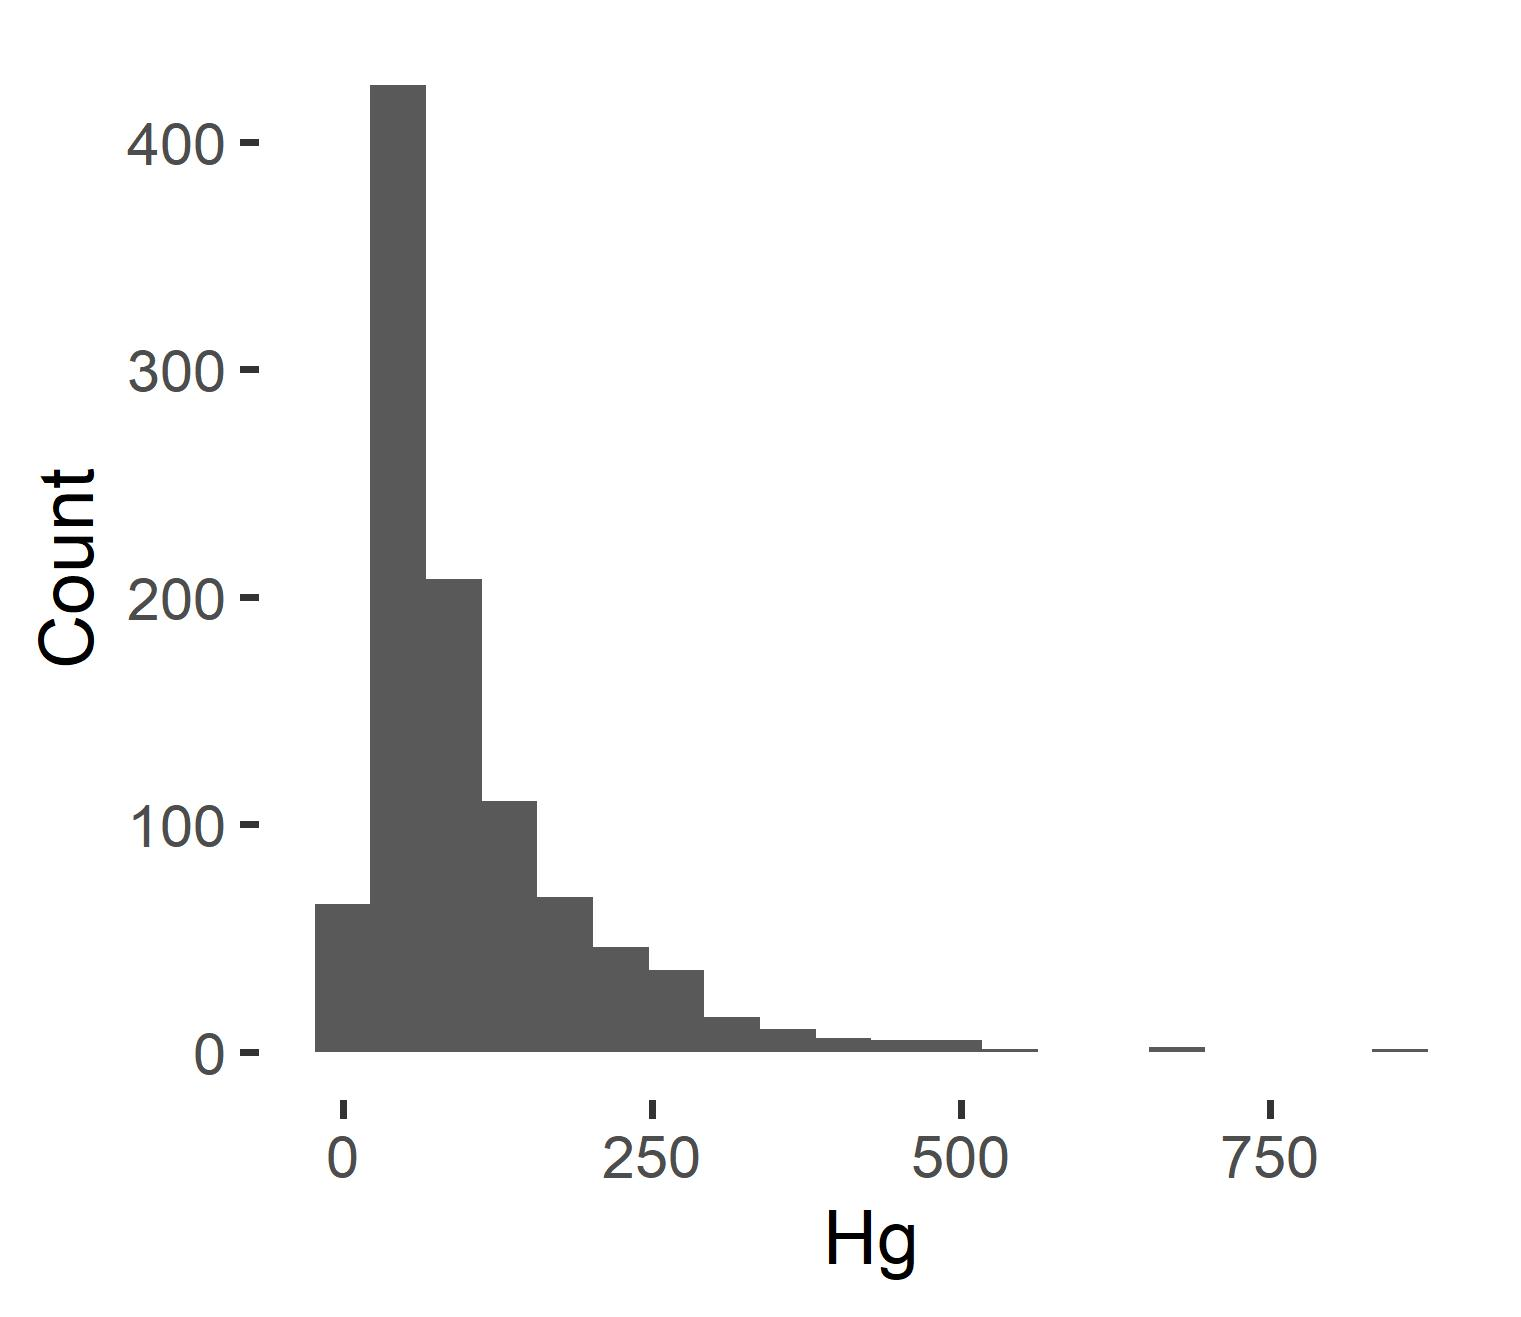
\includegraphics[width = 1\linewidth]{figures/mercury_hist.jpeg}
  \caption*{}
  \label{fig:mercury_hist}
\end{subfigure}
\begin{subfigure}{0.49\textwidth}
  \centering
  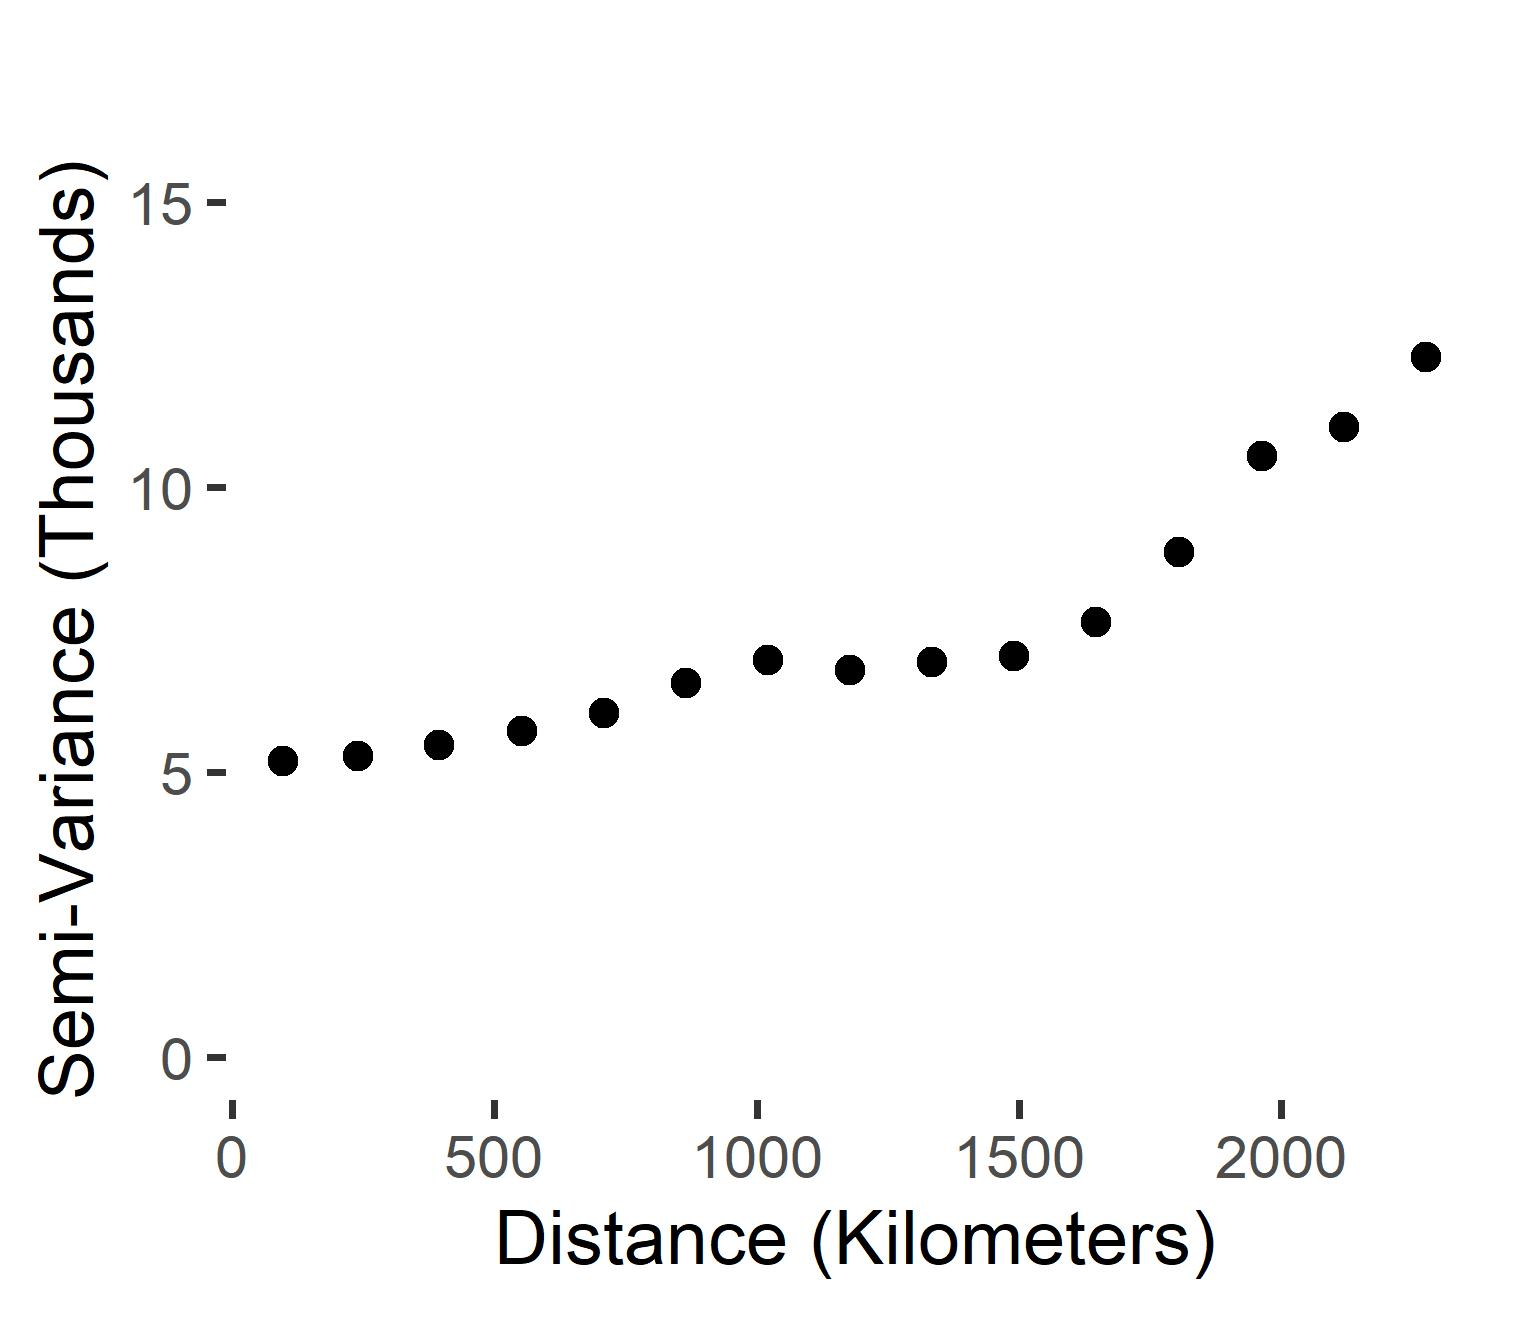
\includegraphics[width = 1\linewidth]{figures/sv_plot.jpeg}
  \caption*{}
  \label{fig:sv_plot}
\end{subfigure}
\caption{Mercury concentration (Hg) visualizations for all 986 lakes in the NLA data. A spatial layout is in the top row, a histogram is in the bottom row and left column, and an empirical semivariogram is in the bottom row and right column.}
\label{fig:merc}
\end{figure}

We selected a single IRS sample and a single GRTS sample and estimated
(design-based) or predicted (model-based) the mean mercury concentration
and constructed 95\% confidence (design-based) and 95\% (model-based)
prediction intervals. For the model-based analyses, the exponential
covariance was used. Table \ref{tab:appliedtab} shows the results from
these analyses. Though we should not generalize these results to other
samples from this population, we do mention a few findings. First,
IRS-Design has the largest standard error. Second, compared to
IRS-Design and IRS-Model, GRTS-Design and GRTS-Model are much closer to
the true mean mercury concentration (have bias closer to zero) and have
much lower standard errors (more precise intervals). Third, GRTS-Model
has the least amount of bias and the lowest standard error (most precise
interval). Finally, we note that for all sampling-analysis combinations,
the true mean mercury concentration (103.2 ng / g) is within the bounds
of the combination's 95\% interval.

\begin{table}[ht]
\centering
\begin{tabular}{lrrrrr}
  \hline
Approach & True Mean & Est/Pred & SE & 95\% LB & 95\% UB \\ 
  \hline
IRS-Design & 103.2 & 112.7 & 8.8 & 95.4 & 129.9 \\ 
  IRS-Model & 103.2 & 110.5 & 7.9 & 95.0 & 125.9 \\ 
  GRTS-Design & 103.2 & 101.8 & 6.1 & 89.8 & 113.7 \\ 
  GRTS-Model & 103.2 & 102.3 & 5.9 & 90.8 & 113.9 \\ 
   \hline
\end{tabular}
\caption{\label{tab:appliedtab} For each sampling-analysis combination (Approach), the true mean mercury concentration (True Mean), estimates/predictions (Est/Pred), standard errors (SE), lower 95\% interval bounds (95\% LB), and upper 95\% interval bounds (95\% UB) for mean mercury concentration computed using a sample of 100 lakes in the NLA data.} 
\end{table}

\hypertarget{new-application}{%
\subsection{New Application}\label{new-application}}

\begin{figure}
\centering
\begin{subfigure}{0.98\textwidth}
  \centering
  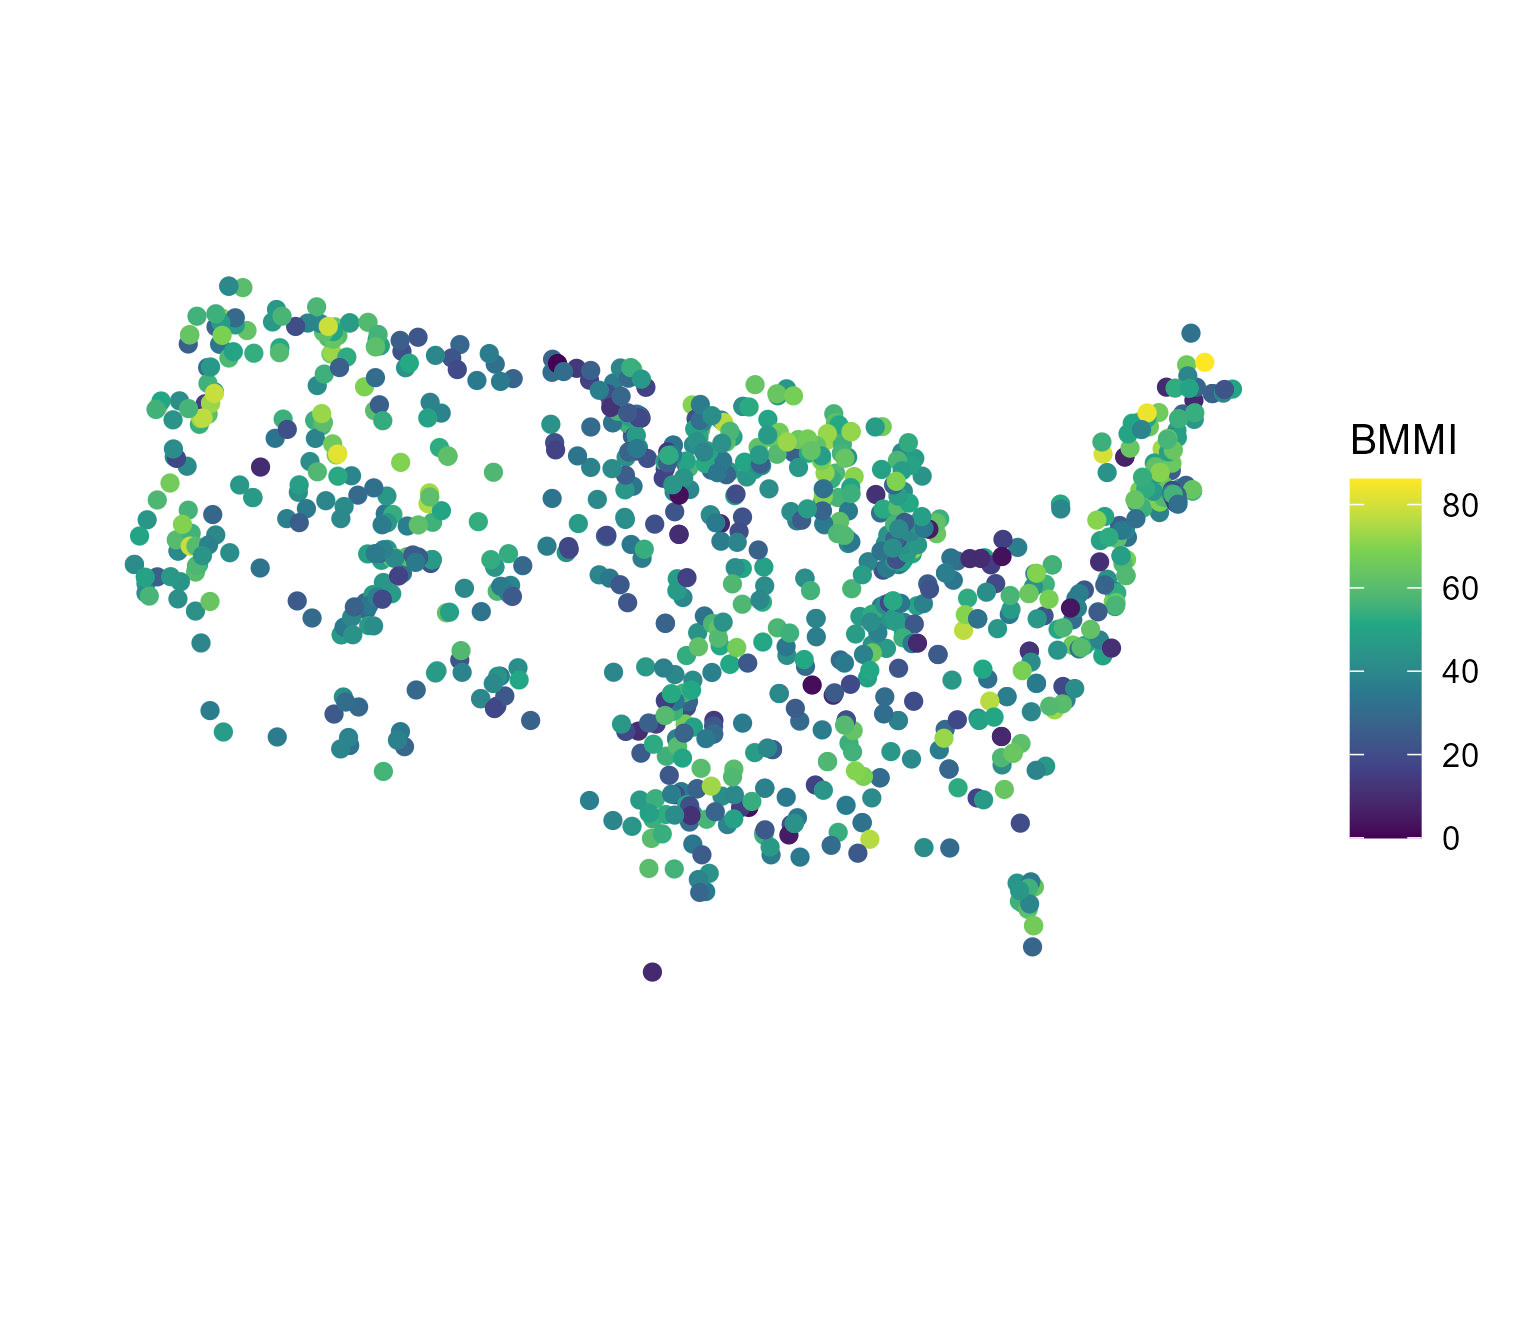
\includegraphics[width = 1\linewidth]{figures/bmmi_map.jpeg}
  \caption*{}
  \label{fig:bmmi_map}
\end{subfigure} \\
\begin{subfigure}{0.49\textwidth}
  \centering
  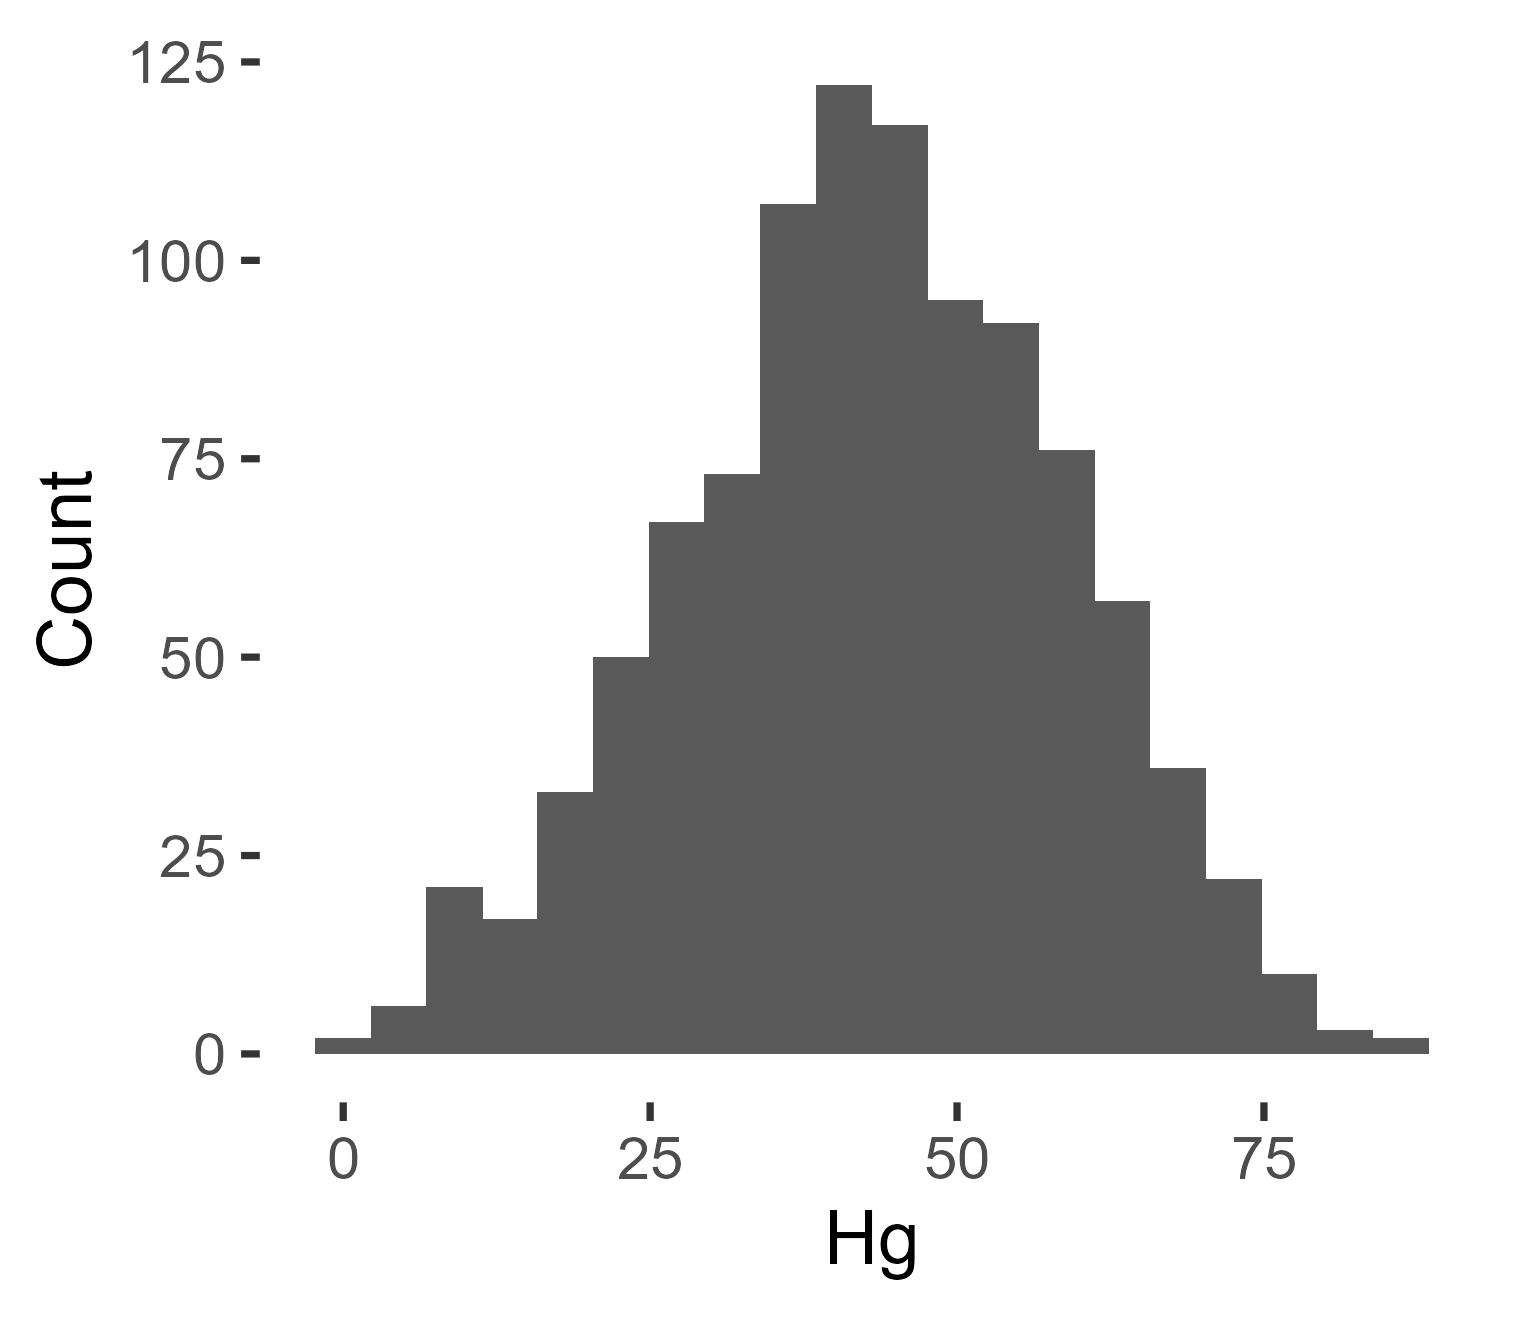
\includegraphics[width = 1\linewidth]{figures/bmmi_hist.jpeg}
  \caption*{}
  \label{fig:bmmi_hist}
\end{subfigure}
\begin{subfigure}{0.49\textwidth}
  \centering
  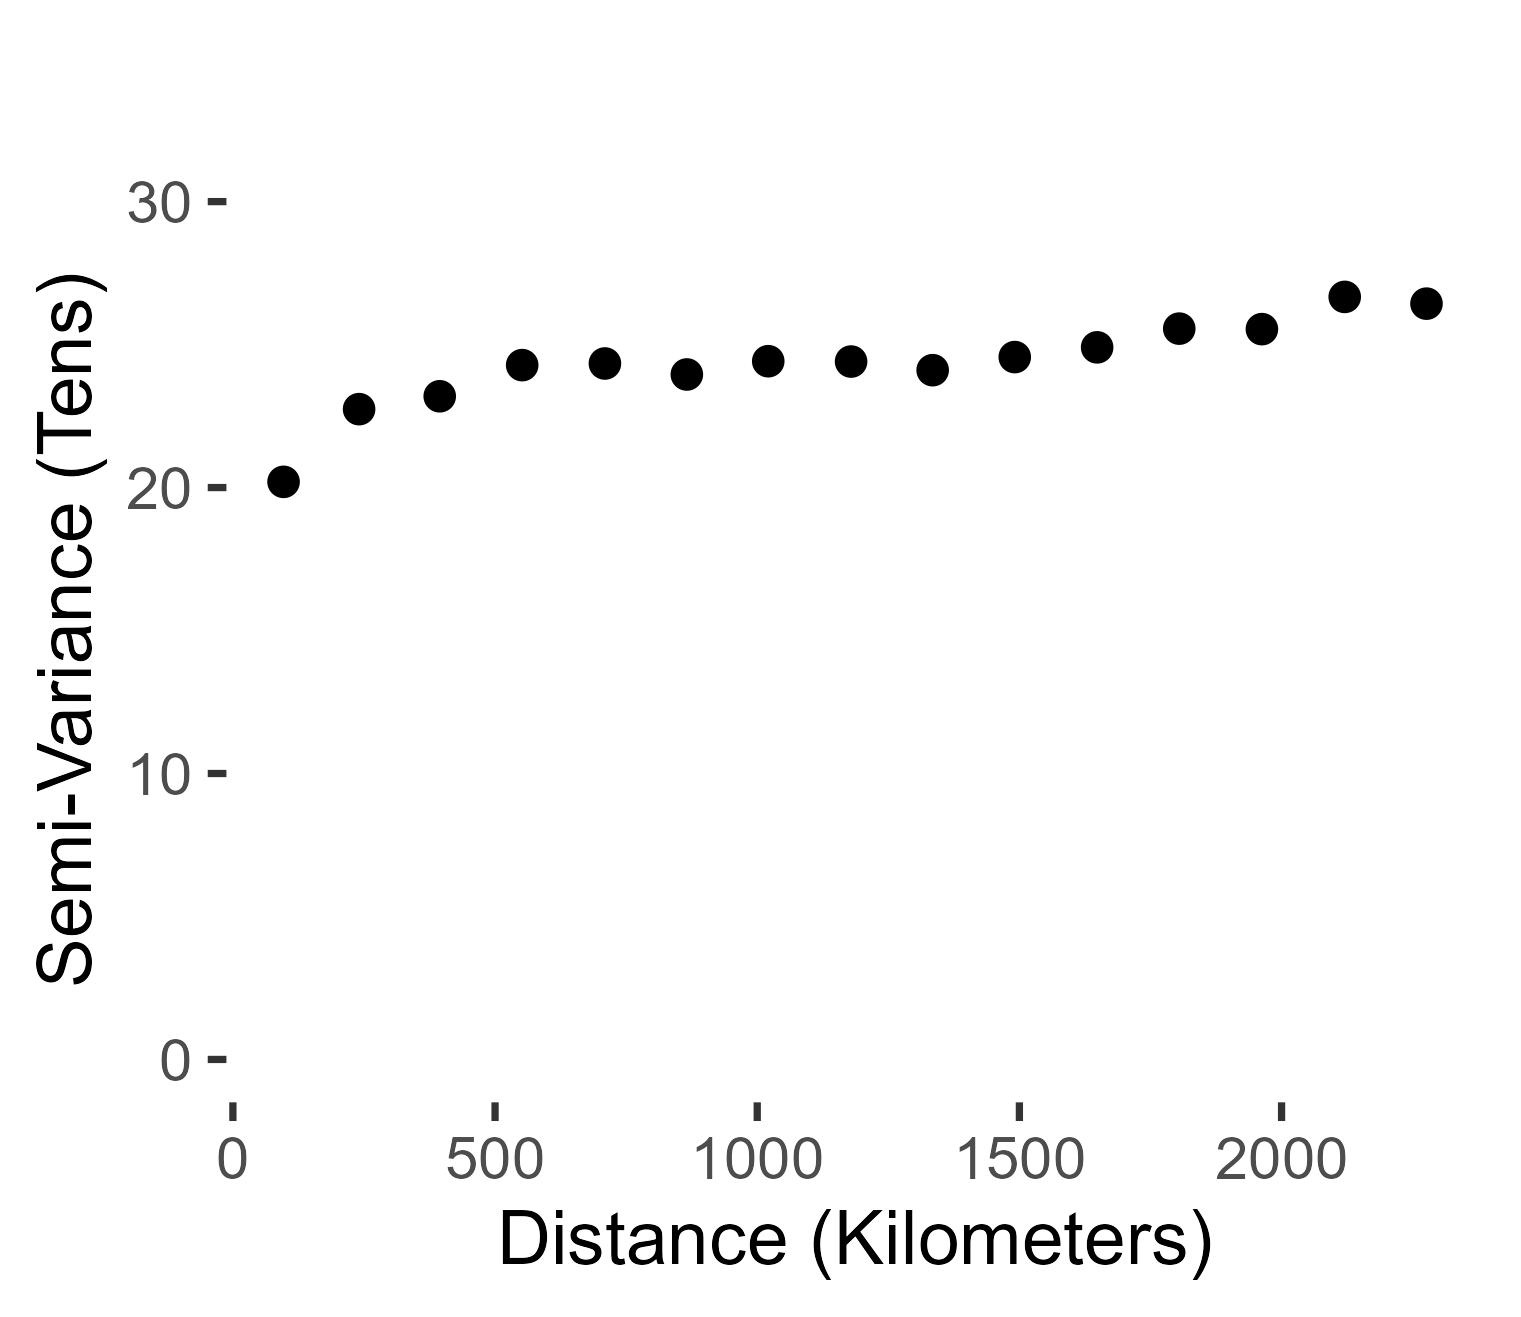
\includegraphics[width = 1\linewidth]{figures/bmmi_sv_plot.jpeg}
  \caption*{}
  \label{fig:bmmi_sv_plot}
\end{subfigure}
\caption{BMMI visualizations for all 986 lakes in the NLA data. A spatial layout is in the top row, a histogram is in the bottom row and left column, and an empirical semivariogram is in the bottom row and right column.}
\label{fig:merc}
\end{figure}

\begin{figure}
  \centering
  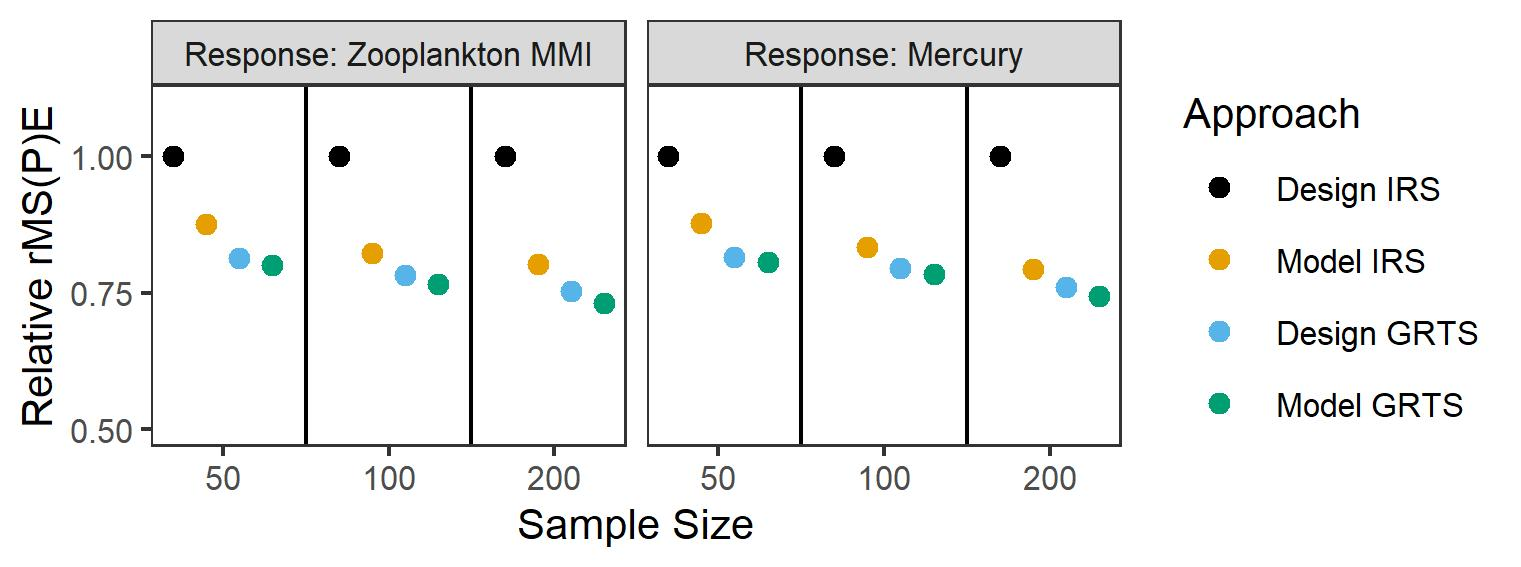
\includegraphics[width = 1\linewidth]{figures/data_rmspe_eff.jpeg}
  \caption{Relative rMS(P)E in the data study for the four sampling-analysis combinations. The rows indicate the proportion of dependent error and the columns indicate the response type.}
  \label{fig:rmspe_eff}
\end{figure}

\begin{figure}
  \centering
  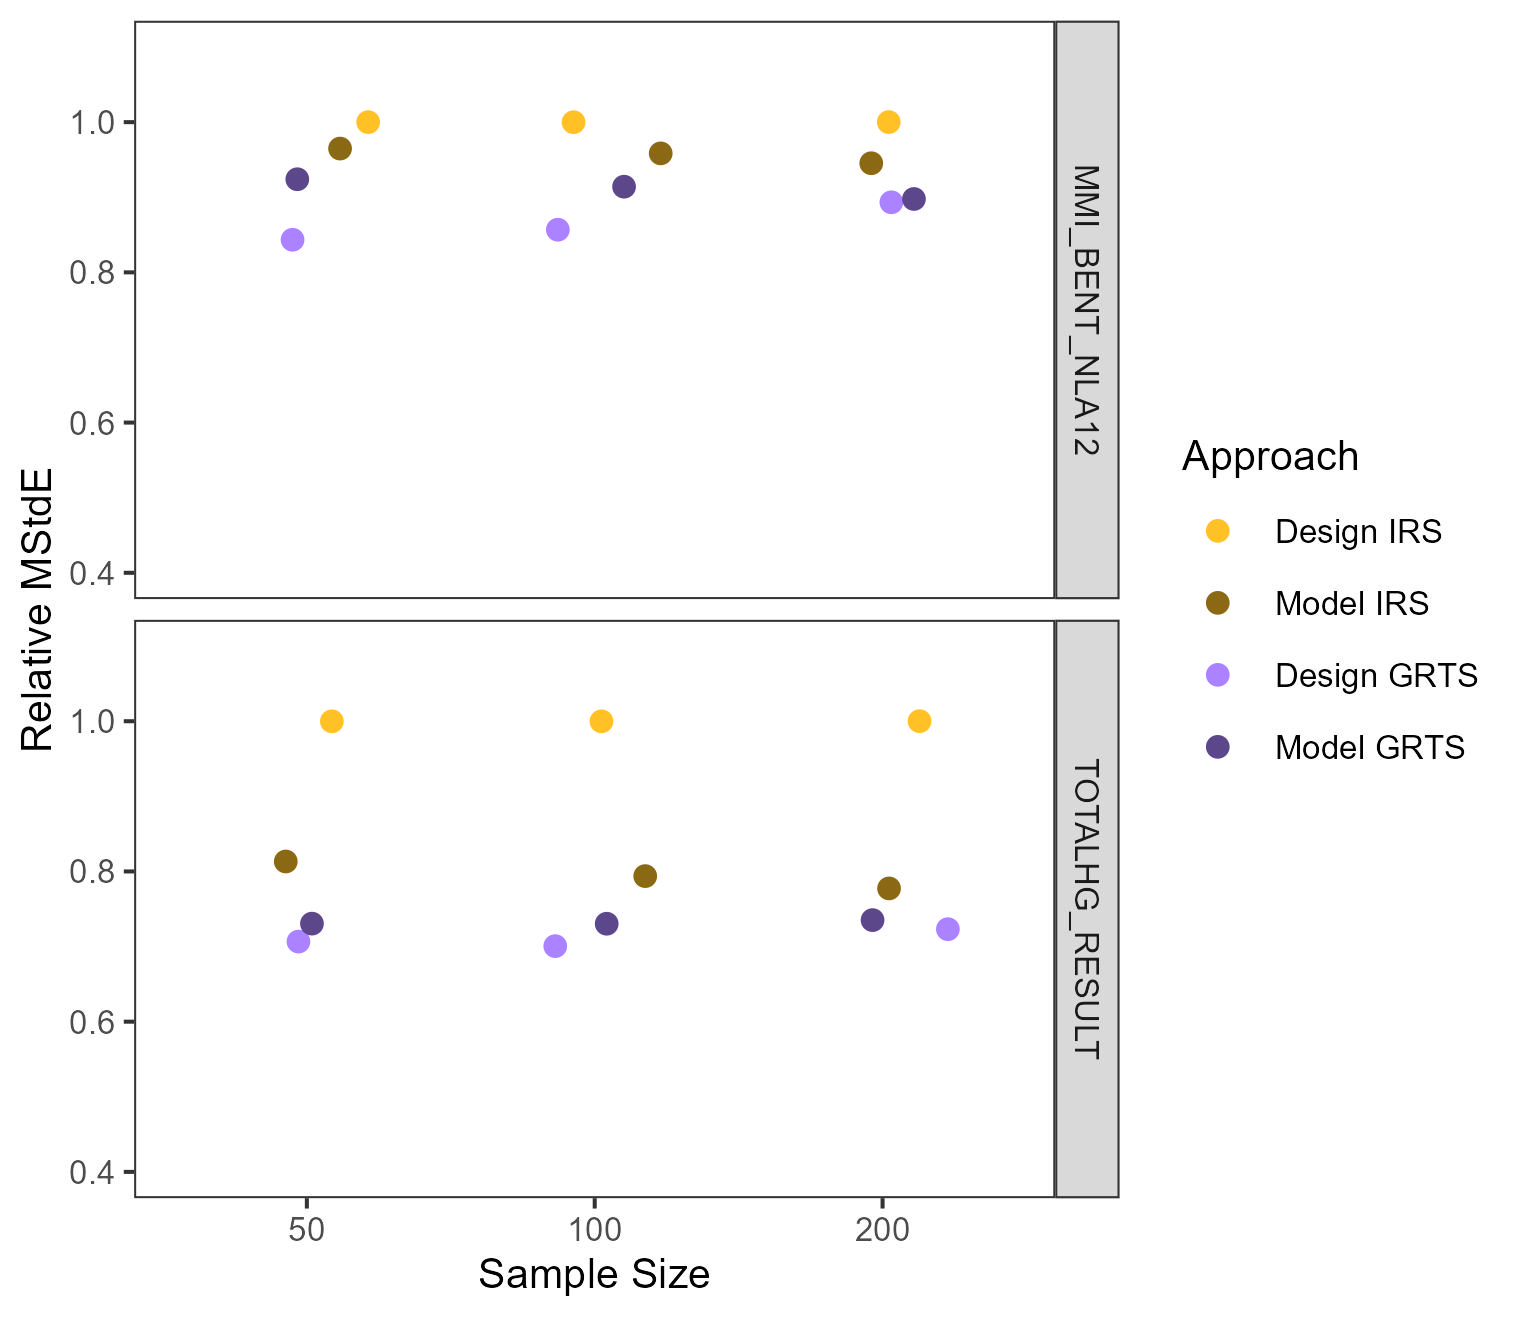
\includegraphics[width = 1\linewidth]{figures/data_mse_eff.jpeg}
  \caption{Relative MStdE in the data study for the four sampling-analysis combinations. The rows indicate the proportion of dependent error and the columns indicate the response type.}
  \label{fig:mse_eff}
\end{figure}

\begin{figure}
  \centering
  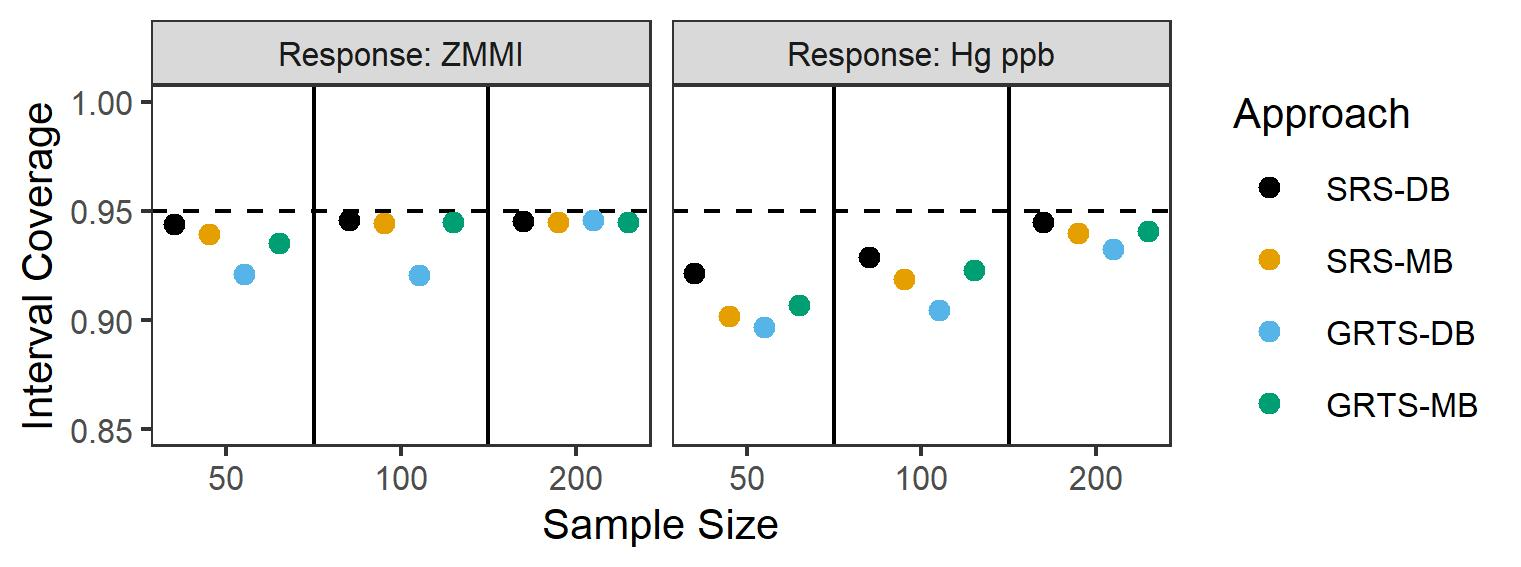
\includegraphics[width = 1\linewidth]{figures/data_coverage.jpeg}
  \caption{Interval coverage in the data study for the four sampling-analysis combinations. The rows indicate the proportion of dependent error and the columns indicate the response type. The solid, black line represents 95\% coverage.}
  \label{fig:figconf}
\end{figure}

\hypertarget{sec:discussion}{%
\section{Discussion}\label{sec:discussion}}

The design-based and model-based approaches to statistical inference are
fundamentally different paradigms. The design-based approach relies on
random sampling to estimate population parameters. The model-based
approach relies on distributional assumptions to predict realized values
of a stochastic process. Though the model-based approach does not rely
on random sampling, it can still be beneficial as a way to guard against
preferential sampling. While the design-based and model-based approaches
have often been compared in the literature from theoretical and
analytical perspectives, our contribution lies in studying them in a
spatial context while implementing spatially balanced sampling and the
design-based, local neighborhood variance estimator. Aside from the
theoretical differences described, a few analytical findings from the
simulation study are particularly notable. First, independent of the
analysis approach, we found no reason to prefer IRS over GRTS when
sampling spatial data -- GRTS-Design and GRTS-Model generally had
similar rMS(P)E as their IRS counterparts when there was no spatial
covariance and lower rMS(P)E than their IRS counterparts when there was
spatial covariance. Second, the sampling decision (IRS vs GRTS) is most
important when using a design-based analysis. Though GRTS-Model still
had lower rMS(P)E than IRS-Model, the model-based analysis mitigated
most of the rMS(P)E inefficiencies that result from the IRS samples
lacking spatial balance. Third, as the strength of spatial covariance
increases, the gap in rMS(P)E and MStdE between IRS-Design and the other
sampling-analysis combinations also increases, likely because IRS-Design
is the only combination that ignores spatial locations in sampling and
analysis. Fourth and finally, when the response was normal, interval
coverage for all sampling-analysis combinations was usually close to
95\% for all sample sizes; when the response was lognormal, interval
coverage for all sampling-analysis combinations was usually between 90\%
and 95\% and closest to 95\% when \(n = 200\).

There are several benefits and drawbacks of the design-based and
model-based approaches for finite population spatial data. Some we have
discussed, but others we have not, and they are worthy of consideration
in future research. Design-based approaches are often computationally
efficient, while model-based approaches can be computationally
burdensome, especially for likelihood-based estimation methods like REML
that rely on inverting a covariance matrix. The design-based approach
also more naturally handles binary data, free from the more complicated
logistic regression framework commonly used to analyze binary data in a
model-based approach. The model-based approach, however, can more
naturally quantify the relationship between covariates (predictor
variables) and the response variable. The model-based approach also
yields estimated spatial covariance parameters, which help better
understand the dependence structure in the stochastic process of study.
Model selection is also possible using model-based approaches and
criteria such as cross validation, likelihood ratio tests, or AIC
(Akaike, 1974). Model-based approaches are capable of more efficient
small-area estimation than design-based approaches by leveraging
distributional assumptions in areas with few observed units. Model-based
approaches can also compute unit-by-unit predictions at unobserved
locations and use them to construct informative visualizations like
smoothed maps. In short, when deciding whether the design-based or
model-based approach is more appropriate to implement, the benefits and
drawbacks of each approach should be considered alongside the particular
goals of the study.

\hypertarget{acknowledgments}{%
\section*{Acknowledgments}\label{acknowledgments}}
\addcontentsline{toc}{section}{Acknowledgments}

The views expressed in this manuscript are those of the authors and do
not necessarily represent the views or policies of the U.S.
Environmental Protection Agency or the National Oceanic and Atmospheric
Administration. Any mention of trade names, products, or services does
not imply an endorsement by the U.S. government, the U.S. Environmental
Protection Agency, or the National Oceanic and Atmospheric
Administration. The U.S. Environmental Protection Agency and National
Oceanic and Atmospheric Administration do not endorse any commercial
products, services, or enterprises.

\hypertarget{conflict-of-interest-statement}{%
\section*{Conflict of Interest
Statement}\label{conflict-of-interest-statement}}
\addcontentsline{toc}{section}{Conflict of Interest Statement}

There are no conflicts of interest for any of the authors.

\hypertarget{author-contribution-statement}{%
\section*{Author Contribution
Statement}\label{author-contribution-statement}}
\addcontentsline{toc}{section}{Author Contribution Statement}

All authors conceived the ideas; All authors designed the methodology;
MD and MH performed the simulations and analyzed the data; MD and MH led
the writing of the manuscript; All authors contributed critically to the
drafts and gave final approval for publication.

\hypertarget{data-and-code-availability}{%
\section*{Data and Code Availability}\label{data-and-code-availability}}
\addcontentsline{toc}{section}{Data and Code Availability}

This manuscript has a supplementary \textbf{\textsf{R}} package that
contains all of the data and code used in its creation. The
supplementary \textbf{\textsf{R}} package is hosted on GitHub.
Instructions for download at available at

\url{https://github.com/michaeldumelle/DvMsp}.

If the manuscript is accepted, this repository will be archived in
Zenodo.

\hypertarget{supporting-information}{%
\section*{Supporting Information}\label{supporting-information}}
\addcontentsline{toc}{section}{Supporting Information}

In the supporting information, we provide tables of summary statistics
for all 36 simulation scenarios.

\hypertarget{references}{%
\section*{References}\label{references}}
\addcontentsline{toc}{section}{References}

\hypertarget{refs}{}
\begin{CSLReferences}{1}{0}
\leavevmode\hypertarget{ref-akaike1974new}{}%
Akaike, H., 1974. A new look at the statistical model identification.
IEEE Transactions on Automatic Control 19, 716--723.

\leavevmode\hypertarget{ref-barabesi2011sampling}{}%
Barabesi, L., Franceschi, S., 2011. Sampling properties of spatial total
estimators under tessellation stratified designs. Environmetrics 22,
271--278.

\leavevmode\hypertarget{ref-benedetti2017spatially}{}%
Benedetti, R., Piersimoni, F., 2017. A spatially balanced design with
probability function proportional to the within sample distance.
Biometrical Journal 59, 1067--1084.

\leavevmode\hypertarget{ref-benedetti2017spatiallyreview}{}%
Benedetti, R., Piersimoni, F., Postiglione, P., 2017. Spatially balanced
sampling: A review and a reappraisal. International Statistical Review
85, 439--454.

\leavevmode\hypertarget{ref-breiman2001random}{}%
Breiman, L., 2001. Random forests. Machine Learning 45, 5--32.

\leavevmode\hypertarget{ref-brus1997random}{}%
Brus, D., De Gruijter, J., 1997. Random sampling or geostatistical
modelling? Choosing between design-based and model-dased sampling
strategies for soil (with discussion). Geoderma 80, 1--44.

\leavevmode\hypertarget{ref-brus2021statistical}{}%
Brus, D.J., 2021. Statistical approaches for spatial sample survey:
Persistent misconceptions and new developments. European Journal of Soil
Science 72, 686--703.

\leavevmode\hypertarget{ref-chan2020bayesian}{}%
Chan-Golston, A.M., Banerjee, S., Handcock, M.S., 2020. Bayesian
inference for finite populations under spatial process settings.
Environmetrics 31, e2606.

\leavevmode\hypertarget{ref-chiles1999geostatistics}{}%
Chiles, J.-P., Delfiner, P., 1999. Geostatistics: {Modeling Spatial
Uncertainty}. {John Wiley \& Sons}, New York.

\leavevmode\hypertarget{ref-cicchitelli2012model}{}%
Cicchitelli, G., Montanari, G.E., 2012. Model-assisted estimation of a
spatial population mean. International Statistical Review 80, 111--126.

\leavevmode\hypertarget{ref-cooper2006sampling}{}%
Cooper, C., 2006. Sampling and variance estimation on continuous
domains. Environmetrics 17, 539--553.

\leavevmode\hypertarget{ref-cressie1993statistics}{}%
Cressie, N., 1993. Statistics for spatial data. John Wiley \& Sons.

\leavevmode\hypertarget{ref-de1990model}{}%
De Gruijter, J., Ter Braak, C., 1990. Model-free estimation from spatial
samples: A reappraisal of classical sampling theory. Mathematical
Geology 22, 407--415.

\leavevmode\hypertarget{ref-diggle2010geostatistical}{}%
Diggle, P.J., Menezes, R., Su, T., 2010. Geostatistical inference under
preferential sampling. Journal of the Royal Statistical Society: Series
C (Applied Statistics) 59, 191--232.

\leavevmode\hypertarget{ref-dumelle2021spsurvey}{}%
Dumelle, M., Kincaid, T.M., Olsen, A.R., Weber, M.H., 2021. Spsurvey:
Spatial sampling design and analysis.

\leavevmode\hypertarget{ref-fix1989discriminatory}{}%
Fix, E., Hodges, J.L., 1989. Discriminatory analysis. Nonparametric
discrimination: Consistency properties. International Statistical
Review/Revue Internationale de Statistique 57, 238--247.

\leavevmode\hypertarget{ref-foster2017spatially}{}%
Foster, S.D., Hosack, G.R., Lawrence, E., Przeslawski, R., Hedge, P.,
Caley, M.J., Barrett, N.S., Williams, A., Li, J., Lynch, T., others,
2017. Spatially balanced designs that incorporate legacy sites. Methods
in Ecology and Evolution 8, 1433--1442.

\leavevmode\hypertarget{ref-grafstrom2012spatiallypoisson}{}%
Grafström, A., 2012. Spatially correlated poisson sampling. Journal of
Statistical Planning and Inference 142, 139--147.

\leavevmode\hypertarget{ref-grafstrom2013well}{}%
Grafström, A., Lundström, N.L., 2013. Why well spread probability
samples are balanced. Open Journal of Statistics 3, 36--41.

\leavevmode\hypertarget{ref-grafstrom2012spatially}{}%
Grafström, A., Lundström, N.L., Schelin, L., 2012. Spatially balanced
sampling through the pivotal method. Biometrics 68, 514--520.

\leavevmode\hypertarget{ref-grafstrom2018spatially}{}%
Grafström, A., Matei, A., 2018. Spatially balanced sampling of
continuous populations. Scandinavian Journal of Statistics 45, 792--805.

\leavevmode\hypertarget{ref-hansen1983evaluation}{}%
Hansen, M.H., Madow, W.G., Tepping, B.J., 1983. An evaluation of
model-dependent and probability-sampling inferences in sample surveys.
Journal of the American Statistical Association 78, 776--793.

\leavevmode\hypertarget{ref-harville1977maximum}{}%
Harville, D.A., 1977. Maximum likelihood approaches to variance
component estimation and to related problems. Journal of the American
Statistical Association 72, 320--338.

\leavevmode\hypertarget{ref-higham2021sptotal}{}%
Higham, M., Ver Hoef, J., Frank, B., Dumelle, M., 2021. Sptotal:
Predicting totals and weighted sums from spatial data.

\leavevmode\hypertarget{ref-horvitz1952generalization}{}%
Horvitz, D.G., Thompson, D.J., 1952. A generalization of sampling
without replacement from a finite universe. Journal of the American
Statistical Association 47, 663--685.

\leavevmode\hypertarget{ref-lohr2009sampling}{}%
Lohr, S.L., 2009. Sampling: Design and analysis. Nelson Education.

\leavevmode\hypertarget{ref-patterson1971recovery}{}%
Patterson, H.D., Thompson, R., 1971. Recovery of inter-block information
when block sizes are unequal. Biometrika 58, 545--554.

\leavevmode\hypertarget{ref-robertson2013bas}{}%
Robertson, B., Brown, J., McDonald, T., Jaksons, P., 2013. BAS: Balanced
acceptance sampling of natural resources. Biometrics 69, 776--784.

\leavevmode\hypertarget{ref-robertson2018halton}{}%
Robertson, B., McDonald, T., Price, C., Brown, J., 2018. Halton
iterative partitioning: Spatially balanced sampling via partitioning.
Environmental and Ecological Statistics 25, 305--323.

\leavevmode\hypertarget{ref-sarndal2003model}{}%
Särndal, C.-E., Swensson, B., Wretman, J., 2003. Model assisted survey
sampling. Springer Science \& Business Media.

\leavevmode\hypertarget{ref-schabenberger2017statistical}{}%
Schabenberger, O., Gotway, C.A., 2017. Statistical methods for spatial
data analysis. CRC press.

\leavevmode\hypertarget{ref-sen1953estimate}{}%
Sen, A.R., 1953. On the estimate of the variance in sampling with
varying probabilities. Journal of the Indian Society of Agricultural
Statistics 5, 127.

\leavevmode\hypertarget{ref-sterba2009alternative}{}%
Sterba, S.K., 2009. Alternative model-based and design-based frameworks
for inference from samples to populations: From polarization to
integration. Multivariate Behavioral Research 44, 711--740.

\leavevmode\hypertarget{ref-stevens2003variance}{}%
Stevens, D.L., Olsen, A.R., 2003. Variance estimation for spatially
balanced samples of environmental resources. Environmetrics 14,
593--610.

\leavevmode\hypertarget{ref-stevens2004spatially}{}%
Stevens, D.L., Olsen, A.R., 2004. Spatially balanced sampling of natural
resources. Journal of the American Statistical Association 99, 262--278.

\leavevmode\hypertarget{ref-USEPA2012NLA}{}%
USEPA, 2012. National lakes assessment 2012.
https://www.epa.gov/national-aquatic-resource-surveys/national-results-and-regional-highlights-national-lakes-assessment.

\leavevmode\hypertarget{ref-verhoef2002sampling}{}%
Ver Hoef, J., 2002. Sampling and geostatistics for spatial data.
Ecoscience 9, 152--161.

\leavevmode\hypertarget{ref-verhoef2008spatial}{}%
Ver Hoef, J.M., 2008. Spatial methods for plot-based sampling of
wildlife populations. Environmental and Ecological Statistics 15, 3--13.

\leavevmode\hypertarget{ref-ver2013comparison}{}%
Ver Hoef, J.M., Temesgen, H., 2013. A comparison of the spatial linear
model to nearest neighbor (k-NN) methods for forestry applications. PlOS
ONE 8, e59129.

\leavevmode\hypertarget{ref-wang2013design}{}%
Wang, J.-F., Jiang, C.-S., Hu, M.-G., Cao, Z.-D., Guo, Y.-S., Li, L.-F.,
Liu, T.-J., Meng, B., 2013. Design-based spatial sampling: Theory and
implementation. Environmental Modelling \& Software 40, 280--288.

\leavevmode\hypertarget{ref-wang2012review}{}%
Wang, J.-F., Stein, A., Gao, B.-B., Ge, Y., 2012. A review of spatial
sampling. Spatial Statistics 2, 1--14.

\leavevmode\hypertarget{ref-wolfinger1994computing}{}%
Wolfinger, R., Tobias, R., Sall, J., 1994. Computing gaussian
likelihoods and their derivatives for general linear mixed models. SIAM
Journal on Scientific Computing 15, 1294--1310.

\end{CSLReferences}


\end{document}
